% !TeX program = xelatex
\documentclass[11pt,a4paper]{article}

% -------------------------------------------------
% Packages
% -------------------------------------------------
\usepackage{kotex}
\usepackage{fontspec}
\usepackage{amsmath,amssymb,bm,mathtools}
\usepackage[left=24mm,right=24mm,top=23mm,bottom=25mm]{geometry}
\usepackage{booktabs,array}
\usepackage{enumitem}
\usepackage{setspace}
\usepackage{xcolor}
\usepackage{colortbl}
\usepackage{tikz}
\usepackage{pifont}
\usetikzlibrary{positioning,arrows.meta,calc,fit,decorations.pathreplacing}
\usepackage[most]{tcolorbox}
\usepackage{listings}
\usepackage{hyperref}
\usepackage{fancyhdr}

\setstretch{1.14}
\setlength{\parindent}{0pt}
\setlength{\parskip}{0.55em}

% -------------------------------------------------
% Colors and boxes
% -------------------------------------------------
\definecolor{deepblue}{RGB}{34,71,120}
\definecolor{softblue}{RGB}{239,246,253}
\definecolor{softgray}{RGB}{246,247,249}
\definecolor{softgreen}{RGB}{239,249,242}
\definecolor{softyellow}{RGB}{255,249,229}
\definecolor{codegray}{RGB}{248,248,248}

\newtcolorbox{keybox}[1][]{
  colback=softblue,
  colframe=deepblue,
  boxrule=0.7pt,
  arc=2mm,
  title=#1,
  fonttitle=\bfseries
}

\newtcolorbox{thinkbox}[1][]{
  colback=softyellow,
  colframe=orange!70!black,
  boxrule=0.6pt,
  arc=2mm,
  title=#1,
  fonttitle=\bfseries
}

\newtcolorbox{remarkbox}[1][]{
  colback=softgray,
  colframe=black!45,
  boxrule=0.5pt,
  arc=2mm,
  title=#1,
  fonttitle=\bfseries
}

\newtcolorbox{mlbox}[1][]{
  colback=softgreen,
  colframe=green!45!black,
  boxrule=0.6pt,
  arc=2mm,
  title=#1,
  fonttitle=\bfseries
}

% -------------------------------------------------
% Code style
% -------------------------------------------------
\lstdefinestyle{pythonstyle}{
  language=Python,
  backgroundcolor=\color{codegray},
  basicstyle=\ttfamily\small,
  keywordstyle=\bfseries,
  commentstyle=\itshape\color{black!60},
  stringstyle=\color{black!75},
  numbers=left,
  numberstyle=\tiny\color{black!55},
  numbersep=8pt,
  frame=single,
  rulecolor=\color{black!25},
  breaklines=true,
  showstringspaces=false,
  tabsize=4,
  columns=fullflexible,
  keepspaces=true
}
\lstset{style=pythonstyle}

% -------------------------------------------------
% Math commands
% -------------------------------------------------
\newcommand{\R}{\mathbb{R}}
\newcommand{\grad}{\nabla}
\newcommand{\vect}[1]{\bm{#1}}
\newcommand{\T}{^{\mathsf T}}
\newcommand{\loss}{\mathcal{L}}
\newcommand{\sigmoid}{\sigma}
\newcommand{\pd}[2]{\frac{\partial #1}{\partial #2}}
\newcommand{\softmax}{\operatorname{softmax}}

% -------------------------------------------------
% Header / footer
% -------------------------------------------------
\pagestyle{fancy}
\fancyhf{}
\lhead{Introduction to Deep Learning and Practice}
\rhead{Convolutional Neural Networks}
\cfoot{\thepage}
\renewcommand{\headrulewidth}{0.4pt}
\setlength{\headheight}{14pt}

\hypersetup{
  colorlinks=true,
  linkcolor=deepblue,
  urlcolor=deepblue
}

% =================================================
% =================================================
\begin{document}
% =================================================

% ---- drawing helpers for this chapter ----
\def\cellsz{0.5}% size of one cell in the grid figures (cm)
% \numgrid{x}{y}{columns}{list}: a grid of numbers, top-left corner at (x, y)
\newcommand{\numgrid}[4]{%
  \foreach \v [count=\k from 0] in {#4} {%
    \pgfmathtruncatemacro{\rr}{int(\k/#3)}%
    \pgfmathtruncatemacro{\cc}{mod(\k,#3)}%
    \draw[black!55] ({#1+\cc*\cellsz},{#2-\rr*\cellsz}) rectangle ++(\cellsz,-\cellsz);%
    \node[font=\small] at ({#1+\cc*\cellsz+0.5*\cellsz},{#2-\rr*\cellsz-0.5*\cellsz}) {\v};%
  }}
% \cuboid{x}{y}{width}{height}{depth}{color}: a block, front face bottom-left at (x, y)
\newcommand{\cuboid}[6]{%
  \filldraw[fill=#6!25,draw=black!70] ({#1},{#2}) rectangle ++({#3},{#4});%
  \filldraw[fill=#6!40,draw=black!70] ({#1},{#2+#4}) -- ++({0.5*#5},{0.4*#5}) -- ++({#3},0) -- ++({-0.5*#5},{-0.4*#5}) -- cycle;%
  \filldraw[fill=#6!55,draw=black!70] ({#1+#3},{#2}) -- ++({0.5*#5},{0.4*#5}) -- ++(0,{#4}) -- ++({-0.5*#5},{-0.4*#5}) -- cycle;%
}

\begin{center}
{\LARGE\bfseries 합성곱 신경망 (CNN)}\\[0.35em]
{\large 합성곱 계층 $\cdot$ 풀링 계층 $\cdot$ im2col $\cdot$ SimpleConvNet $\cdot$ LeNet과 AlexNet}\\[0.8em]
\end{center}

\vspace{0.4em}

\begin{keybox}[이번 주의 핵심 질문]
지금까지의 신경망은 MNIST의 $28\times28$ 이미지를 길이 $784$의 벡터로 \textbf{펼쳐서} 입력하였다.
그러면 ``이 픽셀의 바로 위와 바로 옆에 어떤 픽셀이 있는가''라는 \textbf{공간 정보}를 신경망이 직접 활용하지 못한다.
이미지의 모양을 그대로 유지한 채 학습하는 방법은 없을까?
그리고 이미지의 어느 위치에 있든 같은 모양(예: 세로 획)을 같은 방법으로 알아보려면 어떻게 해야 할까?
\end{keybox}

\subsection*{학습목표}

이 주차가 끝나면 다음을 설명하고 직접 계산할 수 있어야 한다.

\begin{enumerate}[label=\arabic*.]
\item 완전연결 계층과 비교하여 합성곱 계층이 이미지에 적합한 이유(공간 정보, 가중치 공유)를 설명한다.
\item 합성곱 연산을 손으로 계산하고, 패딩과 스트라이드에 따른 출력 크기를 구한다.
\item 여러 채널, 여러 필터, 미니배치에 대한 합성곱을 4차원 배열의 shape으로 설명한다.
\item 최대 풀링의 계산과 그 특징을 설명한다.
\item im2col을 이용하여 합성곱을 하나의 행렬곱(Affine 계층)으로 바꾸고, 그 역전파를 유도한다.
\item 합성곱 계층과 풀링 계층으로 CNN을 구성하여 MNIST를 학습시키고, 학습된 필터를 해석한다.
\item LeNet과 AlexNet의 구조와 차이를 설명한다.
\end{enumerate}

% =================================================
\section{전체 구조}\label{sec:structure}
% =================================================

\textbf{합성곱 신경망(Convolutional Neural Network, CNN)}은 이미지 인식과 음성 인식 등 다양한 곳에서 쓰이는 신경망이다.
지금까지 본 신경망과 마찬가지로 계층을 조합하여 만들지만,
\textbf{합성곱 계층(convolutional layer)}과 \textbf{풀링 계층(pooling layer)}이라는 새로운 계층이 등장한다.
이 두 계층은 수학에서 먼저 나온 것이 아니라, \textbf{동물의 시각 피질에 대한 실험}에서 출발하였다.

\paragraph{출발점: 고양이의 시각 피질 (Hubel과 Wiesel, 1959--1962).}
Hubel과 Wiesel은 마취한 고양이에게 스크린으로 여러 무늬를 보여 주면서,
뇌의 \textbf{1차 시각 피질}에 꽂은 전극으로 뉴런 \textbf{하나}의 반응(전기 신호, spike)을 기록하였다.
점 무늬로는 반응이 거의 없었는데, 슬라이드를 갈아 끼우다가 슬라이드 가장자리가 만든
\textbf{비스듬한 선}이 지나가는 순간 뉴런이 격렬하게 반응했다는 일화가 유명하다.

\begin{center}
\begin{tikzpicture}[>=Latex]
% the screen with a light bar
\fill[black!85] (0,-1.1) rectangle (2.0,1.1);
\draw[white,line width=2.5pt] (0.75,-0.45) -- (1.25,0.45);
\node[font=\scriptsize,below] at (1.0,-1.1) {스크린의 막대 무늬};
% the cat, looking at the screen
\begin{scope}[shift={(4.2,0)}]
\fill[orange!35,draw=orange!70!black] (-0.55,0.45) -- (-0.35,1.05) -- (-0.05,0.62) -- cycle;
\fill[orange!35,draw=orange!70!black] (0.55,0.45) -- (0.35,1.05) -- (0.05,0.62) -- cycle;
\fill[orange!35,draw=orange!70!black] (0,0) circle (0.72);
\fill[black!80] (-0.38,0.08) ellipse (0.1 and 0.14);
\fill[black!80] (-0.02,0.08) ellipse (0.1 and 0.14);
\fill[pink!80!red] (-0.32,-0.2) -- (-0.18,-0.2) -- (-0.25,-0.3) -- cycle;
\draw[black!60] (-0.3,-0.25) -- (-1.0,-0.15) (-0.3,-0.28) -- (-1.0,-0.38);
% the visual cortex at the back of the head, and the electrode
\fill[red!25,draw=red!70!black] (0.42,0.1) ellipse (0.2 and 0.3);
\draw[thick] (0.5,0.15) -- (1.4,1.0);
\node[font=\scriptsize,align=center,red!70!black] at (0.42,-1.05) {1차 시각 피질\\(뉴런 하나에 전극)};
\end{scope}
\draw[->,dashed,black!50] (2.1,0.1) -- (3.4,0.1);
% the recorder
\draw[thick] (5.6,1.0) -- (6.3,1.0);
\draw[rounded corners=2pt,fill=black!5] (6.3,0.25) rectangle (9.3,1.5);
\draw[black!70] (6.45,0.6) -- (9.15,0.6);
\foreach \t in {6.9,7.25,7.4,7.55,7.8,8.0,8.1,8.35,8.7} \draw[thick,blue!70!black] (\t,0.6) -- (\t,1.3);
\node[font=\scriptsize,align=center] at (7.8,-0.1) {기록된 spike\\(막대가 지날 때 많이 발생)};
\end{tikzpicture}

\small (a) 실험의 개념도. 고양이가 스크린의 막대 무늬를 보는 동안 시각 피질의 뉴런 하나의 반응을 기록한다.
\end{center}

막대의 방향과 위치를 바꾸어 가며 기록한 결과, 성질이 다른 두 종류의 뉴런을 찾았다.
점선 원은 그 뉴런의 \textbf{수용 영역(receptive field)}, 즉 그 뉴런이 담당하는 시야의 좁은 영역이다.

\begin{center}
\begin{tikzpicture}[>=Latex]
\def\many{-0.75,-0.58,-0.42,-0.27,-0.12,0.02,0.17,0.32,0.47,0.62,0.76}
% the four stimuli
\foreach \x/\lab in {2.6/{세로 막대},5.4/{세로 막대\\(위치 이동)},8.2/{가로 막대},11.0/{대각선 막대}} {
  \fill[black!85] ({\x-0.5},-0.5) rectangle ({\x+0.5},0.5);
  \draw[white,dashed,thin] (\x,0) circle (0.36);
  \node[font=\scriptsize,align=center,above] at (\x,0.55) {\lab};
}
\draw[white,line width=2.2pt] (2.6,-0.3) -- (2.6,0.3);
\draw[white,line width=2.2pt] (5.65,-0.3) -- (5.65,0.3);
\draw[white,line width=2.2pt] (7.9,0) -- (8.5,0);
\draw[white,line width=2.2pt] (10.79,-0.21) -- (11.21,0.21);
% spike trains: simple cells (row 1) and complex cells (row 2)
\foreach \y/\lab in {-1.2/{단순 세포\\(simple cell)},-2.3/{복합 세포\\(complex cell)}} {
  \node[font=\small,align=center] at (0.5,{\y+0.2}) {\lab};
  \foreach \x in {2.6,5.4,8.2,11.0} \draw[black!60] ({\x-0.9},\y) -- ({\x+0.9},\y);
}
\foreach \t in \many \draw[thick,blue!70!black] ({2.6+\t},-1.2) -- ({2.6+\t},-0.75);
\draw[thick,blue!70!black] (5.5,-1.2) -- (5.5,-0.75);
\foreach \t in {-0.3,0.4} \draw[thick,blue!70!black] ({11.0+\t},-1.2) -- ({11.0+\t},-0.75);
\foreach \t in \many \draw[thick,blue!70!black] ({2.6+\t},-2.3) -- ({2.6+\t},-1.85);
\foreach \t in \many \draw[thick,blue!70!black] ({5.4+\t},-2.3) -- ({5.4+\t},-1.85);
\foreach \t in {-0.3,0.4} \draw[thick,blue!70!black] ({11.0+\t},-2.3) -- ({11.0+\t},-1.85);
\end{tikzpicture}

\small (b) 막대를 보여 줄 때의 spike (세로 선 하나가 신호 하나). 이 두 뉴런은 모두 세로 방향을 좋아한다.
\end{center}

\begin{itemize}[leftmargin=1.5em]
\item \textbf{단순 세포:} 자기 수용 영역 안의 \textbf{특정 위치에 특정 방향}의 에지가 있을 때만 반응한다.
방향이 같아도 위치가 조금 어긋나면 반응하지 않는다. 2.2절에서 볼 \textbf{Sobel 같은 에지 필터}와 같은 일을 한다.
\item \textbf{복합 세포:} 방향만 맞으면 수용 영역 안에서 \textbf{위치가 조금 달라도} 반응한다.
여러 단순 세포의 출력을 모아 그중 하나라도 반응하면 반응하는 것으로 설명된다. 이것은 \textbf{최대 풀링}과 같은 일이다.
\end{itemize}
두 세포는 따로 있는 것이 아니라 \textbf{단계로 이어져} 있다.
단순 세포는 앞 단계(망막과 시상)에서 온 점 모양의 신호를 일렬로 모아 선분을 만들고,
복합 세포는 방향이 같고 위치가 조금씩 다른 단순 세포 여러 개를 모은다.
즉 \textbf{앞 단계의 출력을 모아 조금 더 복잡하거나 위치에 덜 민감한 특징을 만든다}는 것이
Hubel과 Wiesel이 제안한 \textbf{계층 모델}이다.
이 쌓기는 1차 시각 피질(V1) 다음 영역 (V2, V4, 하측두엽)에서도 계속되어, 뒤로 갈수록 보는 범위가 넓어지고
모서리, 모양, 얼굴과 사물처럼 더 복잡한 대상에 반응한다.
Hubel과 Wiesel은 이 연구로 1981년 노벨 생리의학상을 받았다.

\paragraph{시각 피질에서 CNN으로.}
Fukushima는 이 발견을 그대로 신경망으로 옮긴 \textbf{Neocognitron} (1980)을 만들었다.
단순 세포에 해당하는 S-층과 복합 세포에 해당하는 C-층을 번갈아 쌓아, 위치가 조금 달라도 손글씨 숫자를 알아보았다.
다만 가중치는 역전파가 아닌 자기조직화(비지도) 규칙으로 정하였다.
LeCun은 여기에 \textbf{역전파}와 \textbf{가중치 공유}를 결합하여 지금의 CNN을 만들었고 (1989),
이것이 우편번호와 수표의 손글씨를 읽는 \textbf{LeNet} (1998, \ref{sec:lenet}절)이 되었다.
이후 GPU와 대규모 데이터 (ImageNet)를 만나 2012년 \textbf{AlexNet} (\ref{sec:alexnet}절)으로 딥러닝의 시대를 열었다.

\begin{center}
\begin{tikzpicture}[>=Latex,
  hd/.style={draw,rounded corners=3pt,fill=#1,align=center,font=\small,text width=37mm,minimum height=13mm},
  cl/.style={draw=#1!70!black,fill=#1!15,rounded corners=2pt,align=center,font=\small,text width=37mm,minimum height=10mm},
  ar/.style={->,thick,black!60}]
\node[hd=black!6] (h1) at (0,0)   {\textbf{1959--1962}\\Hubel \& Wiesel\\{\scriptsize 고양이 시각 피질 실험}};
\node[hd=black!6] (h2) at (5.2,0) {\textbf{1980}\\Fukushima\\{\scriptsize Neocognitron}};
\node[hd=black!6] (h3) at (10.4,0){\textbf{1989--1998}\\LeCun\\{\scriptsize CNN, LeNet}};
\draw[ar] (h1) -- (h2); \draw[ar] (h2) -- (h3);
\node[cl=orange] (a1) at (0,-1.6)   {단순 세포\\{\scriptsize 특정 위치·방향의 에지}};
\node[cl=orange] (a2) at (5.2,-1.6) {S-층\\{\scriptsize 특징 추출}};
\node[cl=orange] (a3) at (10.4,-1.6){\textbf{합성곱 계층}\\{\scriptsize 필터 = 학습되는 가중치}};
\node[cl=blue] (b1) at (0,-2.9)   {복합 세포\\{\scriptsize 위치가 조금 달라도 반응}};
\node[cl=blue] (b2) at (5.2,-2.9) {C-층\\{\scriptsize 위치 변화 흡수}};
\node[cl=blue] (b3) at (10.4,-2.9){\textbf{풀링 계층}\\{\scriptsize 최대 풀링}};
\draw[ar] (a1) -- (a2); \draw[ar] (a2) -- (a3);
\draw[ar] (b1) -- (b2); \draw[ar] (b2) -- (b3);
\node[font=\scriptsize,align=center,text width=40mm] at (0,-4.0)   {계층 구조\\(단순 $\to$ 복잡)};
\node[font=\scriptsize,align=center,text width=40mm] at (5.2,-4.0) {S-층과 C-층을 번갈아 쌓음\\학습: 자기조직화 (비지도)};
\node[font=\scriptsize,align=center,text width=40mm] at (10.4,-4.0){합성곱과 풀링을 번갈아 쌓음\\학습: \textbf{역전파}, \textbf{가중치 공유}};
\end{tikzpicture}

\small CNN의 계보. 같은 행의 상자는 같은 역할을 한다: 단순 세포 $\to$ S-층 $\to$ 합성곱 계층, 복합 세포 $\to$ C-층 $\to$ 풀링 계층.
\end{center}

고양이 사진을 볼 때 우리는 $13$만 개의 픽셀을 한꺼번에 비교하지 않는다.
먼저 눈, 귀, 코, 수염 같은 \textbf{부분}을 알아보고, 그 부분들이 제자리에 모여 있으니 고양이라고 판단한다.
이때 각 부분은 사진 전체가 아니라 \textbf{그 주변의 좁은 영역}만 보면 알아볼 수 있다.

\IfFileExists{figures/cat_full.png}{%
\begin{center}
\begin{tikzpicture}[>=Latex,
  part/.style={line width=1.4pt},
  crop/.style={inner sep=0pt,draw,line width=1.4pt},
  stage/.style={draw,rounded corners=3pt,fill=black!4,align=center,font=\small,minimum height=11mm,text width=34mm}]
\def\s{0.013304}% cm per pixel: the photo (451 x 300 pixels) is 6 cm wide
\node[anchor=south west,inner sep=0pt] at (0,0) {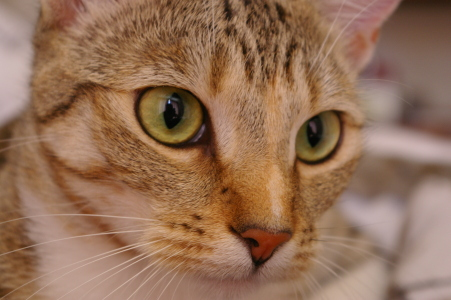
\includegraphics[width=6cm]{figures/cat_full.png}};
% boxes on the photo: (x0, y0, x1, y1) in pixels, the same as in cat_parts.py
\draw[part,blue!80!black]   ({325*\s},{(300-0)*\s})   rectangle ({405*\s},{(300-80)*\s});
\draw[part,red!80!black]    ({130*\s},{(300-80)*\s})  rectangle ({215*\s},{(300-165)*\s});
\draw[part,orange!90!black] ({222*\s},{(300-205)*\s}) rectangle ({307*\s},{(300-290)*\s});
\draw[part,green!50!black]  ({20*\s},{(300-205)*\s})  rectangle ({105*\s},{(300-290)*\s});
% the parts, enlarged
\node[crop,blue!80!black]   (ear)  at (7.6,3.45) {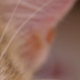
\includegraphics[width=1.05cm]{figures/cat_ear.png}};
\node[crop,red!80!black]    (eye)  at (7.6,2.15) {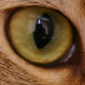
\includegraphics[width=1.05cm]{figures/cat_eye.png}};
\node[crop,orange!90!black] (nose) at (7.6,0.85) {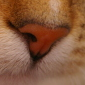
\includegraphics[width=1.05cm]{figures/cat_nose.png}};
\node[crop,green!50!black]  (whi)  at (7.6,-0.45) {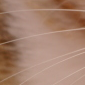
\includegraphics[width=1.05cm]{figures/cat_whisker.png}};
\draw[dashed,blue!80!black]   ({405*\s},{(300-40)*\s})  -- (ear.west);
\draw[dashed,red!80!black]    ({215*\s},{(300-122)*\s}) -- (eye.west);
\draw[dashed,orange!90!black] ({307*\s},{(300-248)*\s}) -- (nose.west);
\draw[dashed,green!50!black]  ({62*\s},{(300-290)*\s})  -- (whi.west);
\node[right=1mm of ear,font=\small]  (lear)  {귀};
\node[right=1mm of eye,font=\small]  (leye)  {눈};
\node[right=1mm of nose,font=\small] (lnose) {코};
\node[right=1mm of whi,font=\small]  (lwhi)  {수염};
% the whole
\node[draw,rounded corners=4pt,fill=orange!15,font=\bfseries,minimum width=17mm,minimum height=10mm] (cat) at (11.2,1.5) {고양이!};
\foreach \p in {lear,leye,lnose,lwhi} \draw[->,thick,black!60] ([xshift=1mm]\p.east) -- (cat.west);
% the hierarchy
\node[stage] (s1) at (1.9,-2.1) {\textbf{작은 영역}\\에지, 색, 질감\\[1pt]{\scriptsize (앞쪽 합성곱 계층)}};
\node[stage] (s2) at (6.4,-2.1) {\textbf{부분}\\눈, 귀, 코, 수염\\[1pt]{\scriptsize (깊은 합성곱 계층)}};
\node[stage] (s3) at (10.9,-2.1) {\textbf{전체}\\고양이\\[1pt]{\scriptsize (완전연결 계층, Softmax)}};
\draw[->,thick] (s1) -- (s2);
\draw[->,thick] (s2) -- (s3);
\end{tikzpicture}

\end{center}
}{%
\begin{center}
\fbox{\parbox{0.8\textwidth}{\centering\small
[그림 자리] \texttt{figures/cat\_full.png} 등\\
\texttt{cat\_parts.py}를 실행하면 생성된다.}}
\end{center}
}

CNN은 이 과정을 모델링 한다.
\begin{itemize}[leftmargin=1.5em]
\item \textbf{좁은 영역씩 본다:} 합성곱 계층의 출력 하나는 입력의 작은 영역 (예: $3\times3$, $5\times5$)에만 연결된다.
\item \textbf{같은 검출기를 어디에나 쓴다:} ``눈 검출기''는 왼쪽 눈에도 오른쪽 눈에도 쓸 수 있어야 한다.
그래서 하나의 필터를 이미지의 모든 위치로 밀면서 적용한다.
\item \textbf{단순한 것에서 복잡한 것으로:} 앞쪽 계층은 에지나 색 같은 단순한 무늬를 찾고,
뒤쪽 계층은 앞에서 찾은 무늬를 조합하여 눈, 귀 같은 부분을, 마지막의 완전연결 계층은 부분들을 모아 ``고양이''를 판단한다.
\end{itemize}
이 세 가지가 이번 주에 배울 합성곱 계층의 국소 연결, 가중치 공유, 그리고 계층을 쌓는 구조이다.

이것을 신경망의 모양으로 그리면 다음과 같다.
입력 이미지의 작은 영역이 필터(빨간 상자, 가중치)와 곱해져 합이 계산되고(합성곱) 그 값이 다음 특징 맵의 한 점이 되고,
합성곱과 풀링을 거듭할 때마다 특징 맵은 작아지는 대신 개수(채널)가 많아진다.이때 각각의 필터는 각 특징을 추출하는 가중치 행렬이다.
마지막 특징 맵을 한 줄로 펼친 뒤에는 지금까지 배운 완전연결 계층과 Softmax로 분류한다.

\IfFileExists{figures/cat_full.png}{%
\begin{center}
\begin{tikzpicture}[>=Latex,scale=0.92,
  fmb/.style={draw=blue!60!black,fill=blue!30,line width=0.5pt},
  fmg/.style={draw=green!60!black,fill=green!30,line width=0.5pt},
  fmy/.style={draw=yellow!60!black,fill=yellow!30,line width=0.5pt},
  fmo/.style={draw=orange!60!black,fill=orange!30,line width=0.5pt},
  kb/.style={draw=red!80!black,thick},
  dl/.style={dashed,thick,black!70},
  nn/.style={draw=blue!60!black,fill=blue!25,circle,minimum size=4mm,inner sep=0pt},
  lab/.style={font=\scriptsize,align=center},
  brc/.style={decorate,decoration={brace,mirror,amplitude=5pt},thick,black!60,text=black}]
% input image and the filter window
\node[inner sep=0pt,draw=black!40] at (0.95,0) {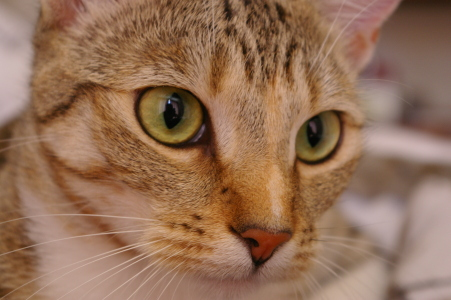
\includegraphics[width=1.9cm]{figures/cat_full.png}};
\draw[kb] (1.15,-0.05) rectangle (1.45,0.25);
% convolution 1: 4 feature maps
\foreach \k in {3,2,1,0} \draw[fmb] ({2.8+\k*0.13},{-0.9+\k*0.13}) rectangle ++(1.8,1.8);
\draw[dl] (1.45,0.25) -- (3.4,0.1);  \draw[dl] (1.45,-0.05) -- (3.4,0.1);
\fill[red!80!black] (3.4,0.1) circle (1.6pt);
\draw[kb] (3.9,-0.45) rectangle ++(0.35,0.35);
% pooling 1: smaller maps, the same number
\foreach \k in {3,2,1,0} \draw[fmg] ({5.6+\k*0.12},{-0.6+\k*0.12}) rectangle ++(1.2,1.2);
\draw[dl] (4.25,-0.1) -- (6.1,-0.2);  \draw[dl] (4.25,-0.45) -- (6.1,-0.2);
\fill[red!80!black] (6.1,-0.2) circle (1.6pt);
\draw[kb] (6.35,0.0) rectangle ++(0.3,0.3);
% convolution 2: more feature maps
\foreach \k in {6,5,...,0} \draw[fmy] ({7.9+\k*0.1},{-0.6+\k*0.1}) rectangle ++(1.2,1.2);
\draw[dl] (6.65,0.3) -- (8.4,0.1);  \draw[dl] (6.65,0.0) -- (8.4,0.1);
\fill[red!80!black] (8.4,0.1) circle (1.6pt);
\draw[kb] (8.7,-0.45) rectangle ++(0.3,0.3);
% pooling 2
\foreach \k in {6,5,...,0} \draw[fmo] ({10.4+\k*0.09},{-0.4+\k*0.09}) rectangle ++(0.8,0.8);
\draw[dl] (9.0,-0.15) -- (10.75,-0.1);  \draw[dl] (9.0,-0.45) -- (10.75,-0.1);
\fill[red!80!black] (10.75,-0.1) circle (1.6pt);
% flatten -> fully connected -> output
\draw[dl] (11.74,0.94) -- (12.48,1.33);  \draw[dl] (11.2,-0.4) -- (12.48,-1.33);
\foreach \i in {0,...,7} \foreach \j in {-2,...,2} \draw[black!25] (12.72,{1.21-\i*0.38}) -- (13.7,{\j*0.6});
\foreach \j in {-2,...,2} \foreach \o in {-1,0,1} \draw[black!25] (13.7,{\j*0.6}) -- (14.8,{\o*0.6});
\foreach \i in {0,...,7} \draw[draw=black!60,fill=black!20] (12.48,{1.33-\i*0.38}) rectangle ++(0.24,-0.24);
\foreach \j in {-2,...,2} \node[nn] at (13.7,{\j*0.6}) {};
\foreach \o in {-1,0,1} \node[nn,fill=orange!40,draw=orange!80!black] at (14.8,{\o*0.6}) {};
\node[anchor=west,font=\scriptsize] at (15.0,0.6)  {고양이 $0.85$};
\node[anchor=west,font=\scriptsize] at (15.0,0)    {개 $0.10$};
\node[anchor=west,font=\scriptsize] at (15.0,-0.6) {새 $0.05$};
% labels
\node[lab] at (3.9,1.75) {합성곱};
\node[lab] at (6.4,1.75) {풀링};
\node[lab] at (8.9,1.75) {합성곱};
\node[lab] at (11.0,1.75) {풀링};
\node[lab] at (15.5,1.85) {출력};
\node[lab] at (0.95,-1.25) {입력 이미지\\{\color{red!80!black}(빨간 상자: 필터)}};
\node[lab] at (3.7,-1.35) {특징 맵};
\node[lab] at (6.2,-1.35) {풀링된\\특징 맵};
\node[lab] at (8.6,-1.35) {특징 맵\\(채널 증가)};
\node[lab] at (10.85,-1.35) {풀링된\\특징 맵};
\node[lab] at (12.6,1.85) {펼치기\\(Flatten)};
\node[lab] at (13.9,1.85) {완전연결\\계층};
% the three stages
\draw[brc] (2.8,-2.4) -- (11.8,-2.4) node[midway,below=5pt,lab,font=\small] {특징 추출 (합성곱 계층 + 풀링 계층)};
\draw[brc] (12.3,-2.4) -- (14.2,-2.4) node[midway,below=5pt,lab,font=\small] {분류};
\draw[brc] (14.5,-2.4) -- (16.4,-2.4) node[midway,below=5pt,lab,font=\small] {확률 (Softmax)};
\end{tikzpicture}

\small 전형적인 CNN의 구조. 앞부분은 특징을 추출하고, 뒷부분은 지금까지의 신경망으로 분류한다.
\end{center}
}{}

완전연결신경망(FNN)은 인접하는 계층의 모든 node가 연결되어 있었다. 완전연결 계층을 Affine 계층이라는 이름으로 구현하였다.

\begin{center}
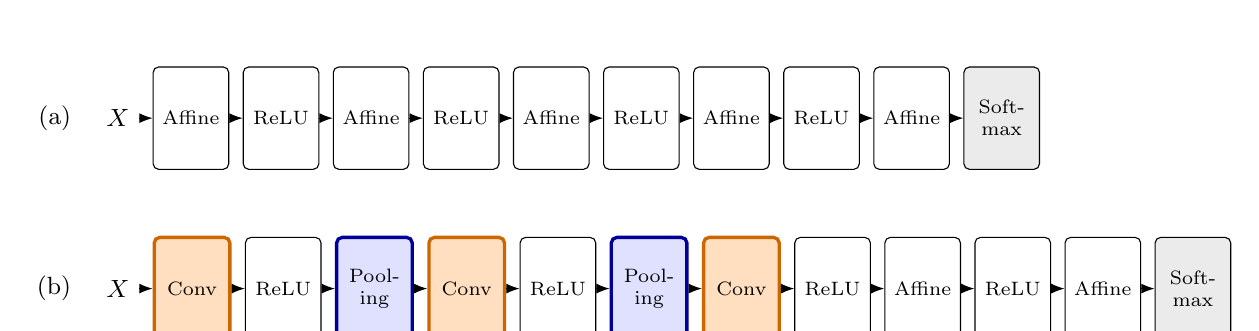
\begin{tikzpicture}[>=Latex,
  lay/.style={draw,rounded corners=2pt,minimum width=9.6mm,minimum height=13mm,
              font=\scriptsize,align=center,inner sep=1pt},
  cv/.style={lay,fill=orange!25,draw=orange!80!black,very thick},
  pl/.style={lay,fill=blue!12,draw=blue!60!black,very thick},
  node distance=1.7mm]
% fully connected
\node[font=\small] (in) {$X$};
\node[lay,right=of in] (a1) {Affine};
\node[lay,right=of a1] (r1) {ReLU};
\node[lay,right=of r1] (a2) {Affine};
\node[lay,right=of a2] (r2) {ReLU};
\node[lay,right=of r2] (a3) {Affine};
\node[lay,right=of a3] (r3) {ReLU};
\node[lay,right=of r3] (a4) {Affine};
\node[lay,right=of a4] (r4) {ReLU};
\node[lay,right=of r4] (a5) {Affine};
\node[lay,right=of a5,fill=black!8] (sm) {Soft-\\max};
\foreach \u/\v in {in/a1,a1/r1,r1/a2,a2/r2,r2/a3,a3/r3,r3/a4,a4/r4,r4/a5,a5/sm}
  \draw[->] (\u) -- (\v);
\node[font=\small,anchor=east] at ([xshift=-2mm]in.west) {(a)};
% CNN
\node[font=\small,below=17mm of in] (in2) {$X$};
\node[cv,right=of in2] (c1) {Conv};
\node[lay,right=of c1] (q1) {ReLU};
\node[pl,right=of q1] (p1) {Pool-\\ing};
\node[cv,right=of p1] (c2) {Conv};
\node[lay,right=of c2] (q2) {ReLU};
\node[pl,right=of q2] (p2) {Pool-\\ing};
\node[cv,right=of p2] (c3) {Conv};
\node[lay,right=of c3] (q3) {ReLU};
\node[lay,right=of q3] (b1) {Affine};
\node[lay,right=of b1] (s1) {ReLU};
\node[lay,right=of s1] (b2) {Affine};
\node[lay,right=of b2,fill=black!8] (sm2) {Soft-\\max};
\foreach \u/\v in {in2/c1,c1/q1,q1/p1,p1/c2,c2/q2,q2/p2,p2/c3,c3/q3,q3/b1,b1/s1,s1/b2,b2/sm2}
  \draw[->] (\u) -- (\v);
\node[font=\small,anchor=east] at ([xshift=-2mm]in2.west) {(b)};
\end{tikzpicture}

\small (a) 완전연결 계층(Affine)으로 이루어진 신경망. (b) CNN의 예:
주황색이 합성곱 계층(Conv), 파란색이 풀링 계층(Pooling)이다.
\end{center}

CNN에서는 ``Affine $\to$ ReLU'' 대신 ``Conv $\to$ ReLU $\to$ (Pooling)''의 흐름이 이어진다
(풀링 계층은 생략하기도 한다).
출력에 가까운 층에서는 지금까지의 ``Affine $\to$ ReLU''를 쓰고, 마지막은 ``Affine $\to$ Softmax''이다.
즉 CNN은 앞부분에서 이미지의 특징을 뽑고, 뒷부분은 지금까지의 신경망으로 분류하는 구조이다.

% =================================================
\section{합성곱 계층}\label{sec:conv}
% =================================================

\subsection{완전연결 계층의 문제점}\label{sec:fcproblem}

완전연결 계층의 문제점은 \textbf{데이터의 형상이 무시된다}는 것이다.
MNIST 이미지는 세로 $28$, 가로 $28$, 채널 $1$ (흑백)인 3차원 데이터 $(1, 28, 28)$이지만,
Affine 계층에 넣으려면 $784$개의 값을 한 줄로 펼쳐야 했다.
이미지에서는 공간적으로 가까운 픽셀끼리 값이 비슷하고, RGB의 세 채널은 서로 밀접하게 관련되어 있으며,
떨어진 픽셀끼리는 관련이 적다. 펼쳐도 값과 순서는 그대로 남아 있지만 (reshape로 되돌릴 수 있다), 완전연결 계층은 이런 \textbf{3차원 모양에 담긴 패턴}을 구조적으로 활용하지 못한다.
완전연결 계층은 모든 입력을 같은 차원의 값으로 취급하므로, 모든 이미지의 픽셀을 같은 순서로 섞어도 표현할 수 있는 함수는 달라지지 않는다.
즉 어느 픽셀이 어느 픽셀의 이웃인지에 대한 가정이 들어 있지 않다.

\begin{center}
\begin{tikzpicture}[>=Latex,
  lb/.style={font=\scriptsize\bfseries,inner sep=0pt},
  brc/.style={decorate,decoration={brace,mirror,amplitude=4pt},thick,black!60}]
\def\s{0.4}% cell size of the image (cm)
\def\t{0.3}% cell size of the flattened vector (cm)
% (a) a 7x7 image of the digit 7: white ink on black, as in MNIST
\foreach \r/\row in {0/{0,1,1,1,1,1,0},1/{0,0,0,0,0,1,0},2/{0,0,0,0,1,0,0},3/{0,0,0,1,0,0,0},
                     4/{0,0,0,1,0,0,0},5/{0,0,1,0,0,0,0},6/{0,0,1,0,0,0,0}} {
  \foreach \v [count=\c from 0] in \row {
    \pgfmathtruncatemacro{\g}{85-85*\v}
    \fill[black!\g] ({\c*\s},{-\r*\s}) rectangle ++(\s,-\s);
    \pgfmathtruncatemacro{\i}{\r*7+\c}
    \fill[black!\g] ({\i*\t},-4.0) rectangle ++(\t,-\t);
  }}
\draw[black!40,step=\s] (0,{-7*\s}) grid ({7*\s},0);
% highlighted pixels: A, its right neighbour B, the pixel below C, a far pixel D
\foreach \r/\c/\col/\n in {3/3/red/A,3/4/cyan/B,4/3/green/C,6/6/orange/D} {
  \draw[\col,line width=1.6pt] ({\c*\s},{-\r*\s}) rectangle ++(\s,-\s);
  \node[lb,\col] at ({\c*\s+0.5*\s},{-\r*\s-0.5*\s}) {\n};
  \pgfmathtruncatemacro{\i}{\r*7+\c}
  \draw[\col,line width=1.6pt] ({\i*\t},-4.0) rectangle ++(\t,-\t);
  \node[lb,\col!70!black] at ({\i*\t+0.5*\t},-3.75) {\n};
}
\node[font=\small,align=center] at ({3.5*\s},-3.15) {(a) 이미지 $(7\times7)$};
% (b) the flattened vector
\foreach \k in {1,...,6} \draw[black!70,thick] ({7*\k*\t},-3.9) -- ({7*\k*\t},-4.4);
\draw[black!40] (0,-4.0) rectangle ({49*\t},{-4.0-\t});
\foreach \k in {1,...,7} \node[font=\tiny,black!60] at ({(7*\k-3.5)*\t},-4.5) {\k 행};
\draw[brc] ({24.5*\t},-4.75) -- ({31.5*\t},-4.75) node[midway,below=4pt,font=\scriptsize,text=black] {A와 C: $7$칸 떨어짐};
\node[font=\small] at ({24.5*\t},-5.55) {(b) 한 줄로 펼친 벡터 $(49)$};
\draw[->,thick,black!60] (3.2,-1.4) .. controls (4.6,-1.8) and (5.4,-2.6) .. ({24.5*\t},-3.6)
  node[pos=0.35,right=2pt,font=\scriptsize,black] {펼치기 (reshape)};
% (c) the three channels of a color image
\foreach \x/\y/\col/\ly in {9.9/0.2/blue/-0.1,9.5/-0.2/green/-2.0,9.1/-0.6/red/-2.4} {
  \fill[\col!15] (\x,\y) rectangle ++({5*\s},{-5*\s});
  \draw[\col!60!black,step=\s,shift={(\x,\y)}] (0,{-5*\s}) grid ({5*\s},0);
  \draw[black,line width=1.4pt] ({\x+2*\s},{\y-2*\s}) rectangle ++(\s,-\s);
}
\foreach \xe/\ly/\col/\n in {11.9/-0.1/blue/B,11.5/-1.95/green/G,11.1/-2.4/red/R} {
  \draw[\col!60!black] (\xe,\ly) -- (12.25,\ly);
  \node[font=\small\bfseries,\col!60!black,right] at (12.25,\ly) {\n};
}
\draw[dashed,thick] ({9.1+2.5*\s},{-0.6-2.5*\s}) -- ({9.9+2.5*\s},{0.2-2.5*\s});
\node[font=\small,align=center] at (10.5,-3.15) {(c) 컬러 이미지의 3채널\\[-1pt]{\scriptsize 같은 위치의 R, G, B}};
\end{tikzpicture}

\small 이미지를 펼치면 드러나지 않는 이웃 관계. (a)에서 A의 바로 옆 B와 바로 아래 C는 모두 A의 이웃이지만,
(b)에서 B만 옆에 남고 C는 한 행의 길이만큼 떨어진다.
\end{center}

그림의 (a)에서 A와 그 이웃 B, C는 서로 가까워 값이 비슷하거나 함께 변하고 (여기서는 A와 C가 같은 획),
멀리 떨어진 D는 A와 관련이 적다. 그러나 (b)처럼 한 줄로 펼치면 A의 오른쪽 이웃 B는 바로 옆에 남지만
아래 이웃 C는 $7$칸 (MNIST라면 $28$칸) 떨어지고, 벡터만 보아서는 C가 A의 이웃이라는 것을 알 수 없다.
(c)의 컬러 이미지에서는 같은 위치의 R, G, B 세 값이 한 점의 색을 함께 이루므로 밀접하게 관련되어 있다.
완전연결 계층은 이런 관계를 모르는 채로 $784$개의 값을 똑같이 다루어, 이웃 관계를 처음부터 데이터로 배워야 한다.

합성곱 계층은 이 \textbf{형상을 유지}한다. 이미지를 3차원 데이터로 입력받고, 다음 계층에도 3차원 데이터로 전달한다.
CNN에서 합성곱 계층의 입출력 데이터를 \textbf{특징 맵(feature map)}이라 한다.
입력 데이터를 \textbf{입력 특징 맵}, 출력 데이터를 \textbf{출력 특징 맵}이라 부른다.

\subsection{합성곱 연산}\label{sec:convop}

합성곱 계층에서는 \textbf{합성곱 연산}을 한다. 이미지 처리에서 말하는 \textbf{필터 연산}이다.

먼저 채널이 하나인 경우를 보자. 입력은 $(4,4)$, 필터는 $(3,3)$이다.
필터를 \textbf{커널(kernel)}이라고도 한다.


\begin{center}
\begin{tikzpicture}
\numgrid{0}{0}{4}{1,2,3,0,0,1,2,3,3,0,1,2,2,3,0,1}
\node[font=\Large] at (2.55,-1) {$\circledast$};
\numgrid{3.1}{-0.25}{3}{2,0,1,0,1,2,1,0,2}
\node[font=\Large] at (5.15,-1) {$\longrightarrow$};
\numgrid{5.8}{-0.5}{2}{15,16,6,15}
\node[font=\small,below] at (1,-2.1) {입력 데이터};
\node[font=\small,below] at (3.85,-2.1) {필터};
\node[font=\small,below] at (6.3,-2.1) {출력};
\end{tikzpicture}
\end{center}

합성곱 연산은 필터의 \textbf{윈도우(window)}를 일정 간격으로 이동해 가며 입력 데이터에 적용한다.
각 위치에서 입력과 필터의 \textbf{대응하는 원소끼리 곱한 뒤 모두 더한다} (곱셈-누산).
수학의 합성곱과 달리 필터를 뒤집지 않으므로 엄밀히는 상호상관(cross-correlation)이지만, 딥러닝에서는 관례적으로 합성곱이라 부른다.
그 결과를 출력의 해당 위치에 저장한다. 왼쪽 위부터 오른쪽 아래까지 모든 위치에서 이 계산을 반복한다.

\begin{center}
\begin{tikzpicture}
\foreach \oi/\oj/\px/\py/\val in {0/0/0/0/15, 0/1/7.6/0/16, 1/0/0/-3.1/6, 1/1/7.6/-3.1/15} {
  \begin{scope}[shift={(\px,\py)}]
    \fill[orange!30] ({\oj*\cellsz},{-\oi*\cellsz}) rectangle ++({3*\cellsz},{-3*\cellsz});
    \numgrid{0}{0}{4}{1,2,3,0,0,1,2,3,3,0,1,2,2,3,0,1}
    \draw[orange!80!black,very thick] ({\oj*\cellsz},{-\oi*\cellsz}) rectangle ++({3*\cellsz},{-3*\cellsz});
    \node at (2.4,-1) {$\circledast$};
    \numgrid{2.85}{-0.25}{3}{2,0,1,0,1,2,1,0,2}
    \node at (4.75,-1) {$\to$};
    \fill[orange!30] ({5.1+\oj*\cellsz},{-0.5-\oi*\cellsz}) rectangle ++(\cellsz,-\cellsz);
    \draw[orange!80!black,very thick] ({5.1+\oj*\cellsz},{-0.5-\oi*\cellsz}) rectangle ++(\cellsz,-\cellsz);
    \draw[black!55] (5.1,-0.5) grid[step=\cellsz] ++({2*\cellsz},{-2*\cellsz});
    \node[font=\small] at ({5.1+\oj*\cellsz+0.5*\cellsz},{-0.5-\oi*\cellsz-0.5*\cellsz}) {\val};
  \end{scope}
}
\end{tikzpicture}

\small 합성곱 연산의 계산 순서. 주황색 윈도우가 왼쪽 위에서 오른쪽 아래로 이동한다.
\end{center}
예를 들어 첫 번째 위치에서는
\[
1\cdot2+2\cdot0+3\cdot1+0\cdot0+1\cdot1+2\cdot2+3\cdot1+0\cdot0+1\cdot2=15
\]
이다. 식으로 쓰면, 입력 $x$와 필터 $f$ ($FH\times FW$)에 대하여 출력의 $(i,j)$ 원소는
\[
y_{ij}=\sum_{p=0}^{FH-1}\sum_{q=0}^{FW-1}x_{i+p,\,j+q}\,f_{pq}
\]
이다.

\paragraph{사람이 설계한 필터: 이미지 처리에서의 특징 추출.}
방금 본 계산, 즉 $3\times3$이나 $5\times5$ 크기의 작은 행렬 (\textbf{필터})을 이미지 위로 한 칸씩 밀면서
대응하는 원소끼리 곱해 모두 더하는 방법은 CNN이 나오기 전부터 이미지 처리에서 특징을 뽑는 데 써 왔다.
어떤 특징을 뽑을지는 필터의 값이 정하고, 그 값은 사람이 목적에 맞게 설계하였다.
대표적인 필터는 다음과 같다.

\begin{center}
\renewcommand{\arraystretch}{1.25}
\begin{tabular}{@{}l c p{0.43\textwidth}@{}}
\toprule
필터 & 값 & 하는 일 \\
\midrule
평균 (blur) & $\dfrac{1}{25}\begin{pmatrix}1&\cdots&1\\ \vdots&\ddots&\vdots\\ 1&\cdots&1\end{pmatrix}_{5\times5}$
& 주변 $25$개 픽셀의 평균. 잡음과 세부가 사라지고 흐려진다. \\[14pt]
선명하게 (sharpen) & $\begin{pmatrix}0&-1&0\\-1&5&-1\\0&-1&0\end{pmatrix}$
& 가운데 픽셀과 이웃의 차이를 키운다. 윤곽이 또렷해진다. \\[14pt]
Sobel $x$ & $\begin{pmatrix}-1&0&1\\-2&0&2\\-1&0&1\end{pmatrix}$
& 오른쪽 열 $-$ 왼쪽 열: 가로 방향 밝기 변화, 즉 \textbf{세로 에지}에 반응한다. \\[14pt]
Sobel $y$ & $\begin{pmatrix}-1&-2&-1\\0&0&0\\1&2&1\end{pmatrix}$
& 아래 행 $-$ 위 행: 세로 방향 밝기 변화, 즉 \textbf{가로 에지}에 반응한다. \\[14pt]
Laplacian & $\begin{pmatrix}0&1&0\\1&-4&1\\0&1&0\end{pmatrix}$
& 이웃의 합 $-$ $4\times$가운데 (2계 미분의 근사): 방향에 관계없이 에지에 반응한다. \\[14pt]
엠보싱 (emboss) & $\begin{pmatrix}-2&-1&0\\-1&1&1\\0&1&2\end{pmatrix}$
& 대각선 방향의 밝기 변화를 더해 돋을새김처럼 보이게 한다. \\
\bottomrule
\end{tabular}
\end{center}

\textbf{왜 이런 필터가 에지에 반응할까?}
왼쪽 절반이 $0$(검정), 오른쪽 절반이 $1$(흰색)인 $5\times5$ 이미지에 Sobel 필터를 적용해 보자.
\begin{center}
\begin{tikzpicture}
\numgrid{0}{-0.95}{5}{0,0,0,1,1,0,0,0,1,1,0,0,0,1,1,0,0,0,1,1,0,0,0,1,1}
\node[font=\Large] at (3.05,-0.75) {$\circledast$};
\numgrid{3.5}{0}{3}{-1,0,1,-2,0,2,-1,0,1}
\node[font=\Large] at (5.45,-0.75) {$\to$};
\numgrid{6.0}{0}{3}{0,4,4,0,4,4,0,4,4}
\node[font=\Large] at (3.05,-3.15) {$\circledast$};
\numgrid{3.5}{-2.4}{3}{-1,-2,-1,0,0,0,1,2,1}
\node[font=\Large] at (5.45,-3.15) {$\to$};
\numgrid{6.0}{-2.4}{3}{0,0,0,0,0,0,0,0,0}
\node[font=\small,below] at (1.25,-3.5) {입력 (세로 에지)};
\node[font=\small,right] at (7.6,-0.75) {Sobel $x$: 에지에서 큰 값};
\node[font=\small,right] at (7.6,-3.15) {Sobel $y$: 모두 $0$};
\end{tikzpicture}
\end{center}
Sobel 필터의 원소를 모두 더하면 $0$이므로, 밝기가 고른 곳에서는 출력이 $0$이다.
Sobel $x$는 창 안에 $0$과 $1$의 경계가 있는 위치에서만 $(0\cdot(-1)+1\cdot1)(1+2+1)=4$를 내고,
같은 이미지에 Sobel $y$를 적용하면 위아래로는 밝기 변화가 없으므로 모두 $0$이다.
즉 출력은 \textbf{그 위치의 이미지 조각이 필터의 무늬와 얼마나 닮았는가}를 나타낸다.
필터의 무늬(왼쪽은 음수, 오른쪽은 양수)와 닮은 곳일수록 곱의 합이 크다.

실제 흑백 사진 ($512\times512$)에 위의 필터들을 적용하면 다음과 같다 (\texttt{classic\_filters.py}).
에지 필터의 출력은 양수와 음수가 모두 나오므로 절댓값을 그렸다 (밝을수록 강한 에지).
마지막 그림은 두 Sobel 출력을 합친 \textbf{에지의 세기}이다.
같은 위치 $(i,j)$에서 Sobel $x$의 출력을 $g_x$, Sobel $y$의 출력을 $g_y$라 하면
(각각 가로 방향과 세로 방향의 밝기 변화량), 그 위치의 에지의 세기는 $\sqrt{g_x^2+g_y^2}$이다.
두 방향의 변화를 벡터 $(g_x,g_y)$로 보고 그 길이를 잰 것이므로, 에지가 어느 방향으로 뻗어 있든 밝게 나타난다.

\IfFileExists{figures/cnn_classic_filters.png}{%
\begin{center}
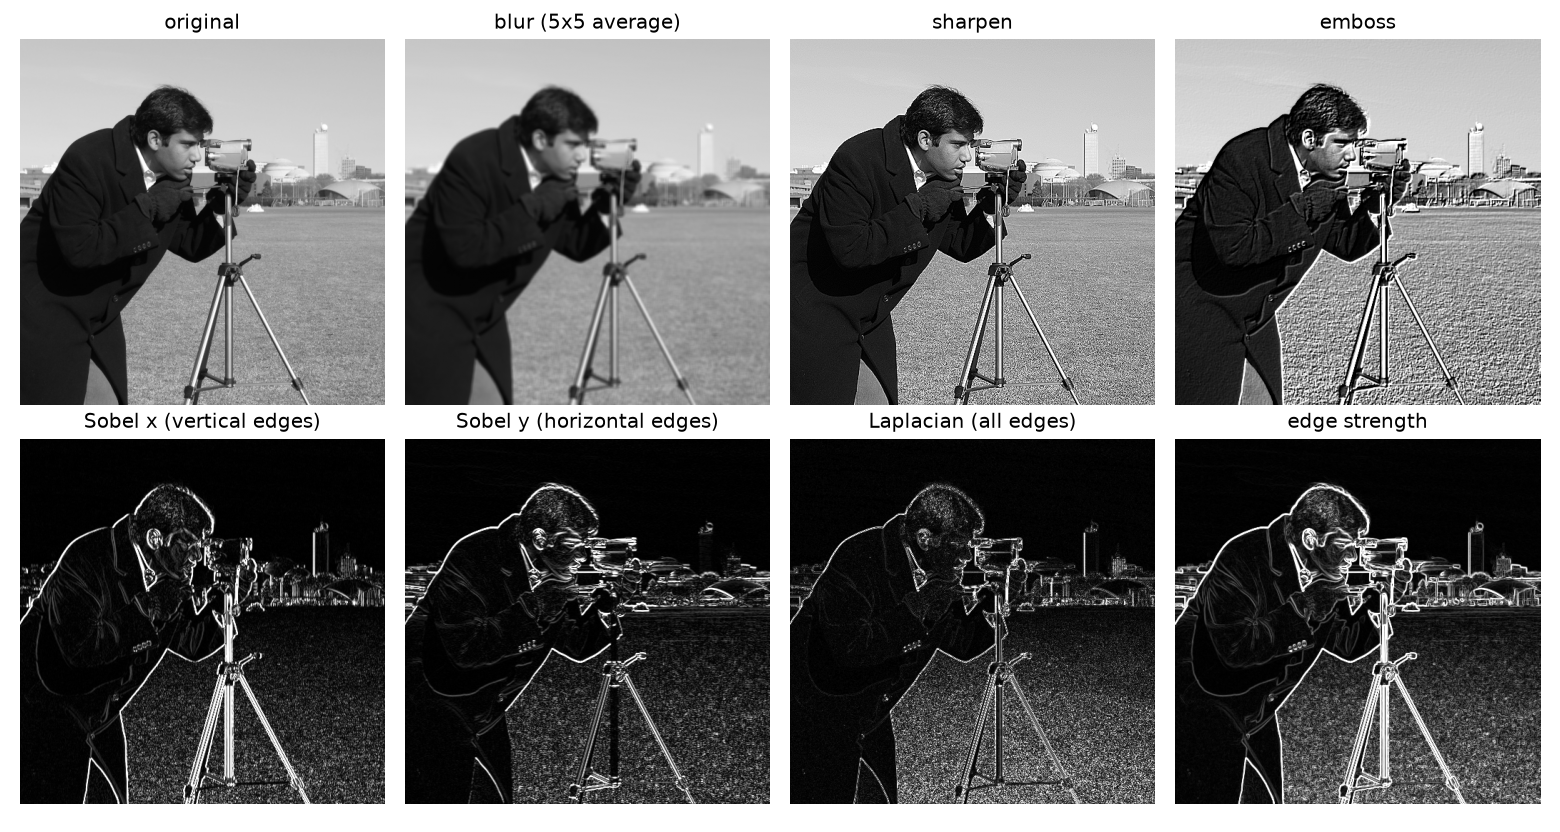
\includegraphics[width=\textwidth]{figures/cnn_classic_filters.png}

\small 사람이 설계한 필터를 흑백 사진에 적용한 결과. 위: 원본, 평균, 선명하게, 엠보싱. 아래: Sobel $x$, Sobel $y$, Laplacian, 에지의 세기.
\end{center}
}{%
\begin{center}
\fbox{\parbox{0.8\textwidth}{\centering\small
[그림 자리] \texttt{figures/cnn\_classic\_filters.png}\\
\texttt{classic\_filters.py}를 실행하면 생성된다.}}
\end{center}
}

두 Sobel 필터의 차이는 확대해 보면 더 분명하다.
Sobel $x$에서는 삼각대 다리와 얼굴의 옆선처럼 \textbf{세로로 뻗은 경계}가 밝고,
Sobel $y$에서는 카메라의 윗면과 아랫면, 지평선처럼 \textbf{가로로 뻗은 경계}가 밝다.
필터 하나가 이미지에서 한 종류의 특징만 골라내는 것이다.

\IfFileExists{figures/cnn_classic_filters_zoom.png}{%
\begin{center}
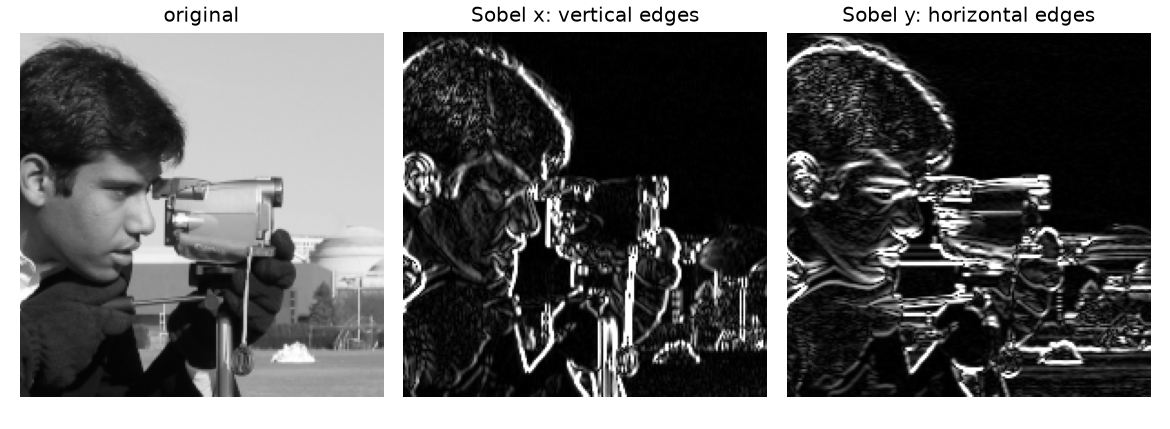
\includegraphics[width=0.9\textwidth]{figures/cnn_classic_filters_zoom.png}

\small 카메라 부분 확대. 같은 위치에서도 필터에 따라 뽑히는 에지의 방향이 다르다.
\end{center}
}{}

\begin{remarkbox}[사람이 설계한 필터는 지금 어디에 쓰이는가]
딥러닝이 대신하게 된 것은 ``이것이 고양이인가'' 같은 복잡한 인식이고,
단순하고 목적이 분명한 처리에는 지금도 고정된 필터가 쓰인다.
\begin{itemize}[leftmargin=1.5em]
\item \textbf{사진·영상 편집과 카메라:} 편집 앱의 ``흐림 효과''와 ``선명하게'', 카메라 내부의 잡음 제거와 윤곽 보정,
이미지를 줄이기 전에 블러를 걸어 계단 현상(앨리어싱)을 막는 처리.
\item \textbf{고전 컴퓨터 비전:} Canny 에지 검출 (가우시안 블러 $\to$ Sobel), Harris 코너 검출 (파노라마 이어 붙이기),
HOG와 SIFT 특징 (기울기 방향의 분포; HOG + SVM 보행자 검출은 2000년대의 대표 기법).
\item \textbf{산업 현장:} 제품 표면의 긁힘 검사, 문서 스캔과 OCR 전처리, 고전적인 차선 인식.
불량 데이터가 적어 학습이 어렵거나, GPU 없는 임베디드 기기처럼 계산 자원이 부족할 때 특히 쓰인다.
\item \textbf{딥러닝 안에서:} 데이터 증강 (무작위 블러, 선명하게), 흐린 사진 걸러내기 (Laplacian 출력의 분산이 작으면 흐린 사진),
이미지 생성·복원 모델의 에지 손실 (Sobel 출력끼리 비교), 풀링 앞에 고정된 블러 필터를 넣는 BlurPool.
\end{itemize}
고정된 필터는 \textbf{데이터가 필요 없고, 해석할 수 있고, 빠르다.}
대신 에지나 블러처럼 사람이 수식으로 정의할 수 있는 특징까지만 다룰 수 있다.
\end{remarkbox}

\begin{keybox}[사람이 설계한 필터에서 학습하는 필터로]
\begin{itemize}[leftmargin=1.5em]
\item 필터 연산은 \textbf{작은 무늬 검출기}이다. 출력은 각 위치에서 그 무늬가 얼마나 강하게 나타나는지를 담은 2차원 지도, 즉 \textbf{특징 맵}이다.
\item 위의 필터들은 사람이 목적에 맞게 값을 정하였다. 그러나 복잡한 이미지를 분류해 내기 위해서 어떤 필터를 적용해야 할지, 어떻게 필터의 값은 정하기는 어렵다.
\item CNN은 필터의 값을 \textbf{데이터로부터 학습}하는 \textbf{가중치로} 취급한다. 즉 필터가 학습 파라미터인 것이다. 학습된 첫 번째 층의 필터도 Sobel처럼 여러 방향의 에지에 반응하고
(\ref{sec:filters}절), 층이 깊어질수록 더 복잡한 무늬를 찾는 필터가 된다 (\ref{sec:depth}절).
\end{itemize}
\end{keybox}

\paragraph{필터가 가중치이다.}
완전연결 신경망에는 가중치 $W$와 편향 $B$가 있었다.
CNN에서는 \textbf{필터의 원소가 가중치}에 해당한다. 필터의 값을 학습하는 것이다.
편향은 필터를 적용한 뒤 모든 원소에 같은 값 하나를 더한다.

\begin{center}
\begin{tikzpicture}
\numgrid{0}{0}{4}{1,2,3,0,0,1,2,3,3,0,1,2,2,3,0,1}
\node[font=\Large] at (2.5,-1) {$\circledast$};
\numgrid{3.0}{-0.25}{3}{2,0,1,0,1,2,1,0,2}
\node[font=\Large] at (5.0,-1) {$\to$};
\numgrid{5.5}{-0.5}{2}{15,16,6,15}
\node[font=\Large] at (7.0,-1) {$+$};
\numgrid{7.5}{-0.75}{1}{3}
\node[font=\Large] at (8.5,-1) {$\to$};
\numgrid{9.0}{-0.5}{2}{18,19,9,18}
\node[font=\small,below] at (3.75,-1.9) {필터 (가중치)};
\node[font=\small,below] at (7.75,-1.9) {편향};
\end{tikzpicture}
\end{center}

\paragraph{합성곱 계층은 연결을 제한한 완전연결 계층이다.}
합성곱 연산을 노드와 화살표로 그리면 완전연결 계층과 비교할 수 있다.
간단히 1차원 입력 $x_1,\ldots,x_6$에 길이 $3$인 필터 $(w_1,w_2,w_3)$를 스트라이드 $1$로 적용하면
출력은 $y_j=w_1x_j+w_2x_{j+1}+w_3x_{j+2}$ ($j=1,\ldots,4$)이다.

\begin{center}
\begin{tikzpicture}[
  nd/.style={draw,circle,minimum size=6.5mm,inner sep=0pt,font=\scriptsize,fill=white},
  ca/.style={blue!70!black,thick}, cb/.style={orange!85!black,thick}, cc/.style={green!50!black,thick}]
% (a) fully connected
\begin{scope}
\foreach \i in {1,...,6} \node[nd] (a\i) at (0,{-0.75*\i}) {$x_\i$};
\foreach \j in {1,...,4} \node[nd] (b\j) at (2.6,{-0.75*(\j+1)}) {$y_\j$};
\foreach \i in {1,...,6} \foreach \j in {1,...,4} \draw[black!45] (a\i) -- (b\j);
\node[font=\small,align=center] at (1.3,-5.45) {(a) 완전연결\\가중치 $6\times4=24$개};
\end{scope}
% (b) convolution
\begin{scope}[xshift=4.6cm]
\foreach \i in {1,...,6} \node[nd] (c\i) at (0,{-0.75*\i}) {$x_\i$};
\foreach \j in {1,...,4} \node[nd] (d\j) at (2.6,{-0.75*(\j+1)}) {$y_\j$};
\foreach \j [evaluate=\j as \ja using int(\j+1), evaluate=\j as \jb using int(\j+2)] in {1,...,4} {
  \draw[ca] (c\j) -- (d\j);
  \draw[cb] (c\ja) -- (d\j);
  \draw[cc] (c\jb) -- (d\j);
}
\node[font=\small,align=center] at (1.3,-5.45) {(b) 합성곱\\가중치 $3$개 (색이 같으면 같은 값)};
\end{scope}
% (c) the weight matrix of (b)
\begin{scope}[xshift=9.4cm,yshift=-1.0cm]
\def\mc{0.52}
\foreach \r in {0,...,5} \foreach \c in {0,...,3} \draw[black!35] ({\c*\mc},{-\r*\mc}) rectangle ++(\mc,-\mc);
\foreach \c in {0,...,3} {
  \pgfmathtruncatemacro{\ra}{\c}\pgfmathtruncatemacro{\rb}{\c+1}\pgfmathtruncatemacro{\rc}{\c+2}
  \fill[blue!20] ({\c*\mc},{-\ra*\mc}) rectangle ++(\mc,-\mc); \node[font=\scriptsize,blue!70!black] at ({(\c+0.5)*\mc},{-(\ra+0.5)*\mc}) {$w_1$};
  \fill[orange!25] ({\c*\mc},{-\rb*\mc}) rectangle ++(\mc,-\mc); \node[font=\scriptsize,orange!85!black] at ({(\c+0.5)*\mc},{-(\rb+0.5)*\mc}) {$w_2$};
  \fill[green!20] ({\c*\mc},{-\rc*\mc}) rectangle ++(\mc,-\mc); \node[font=\scriptsize,green!50!black] at ({(\c+0.5)*\mc},{-(\rc+0.5)*\mc}) {$w_3$};
}
\foreach \r in {0,...,5} \foreach \c in {0,...,3} \draw[black!35] ({\c*\mc},{-\r*\mc}) rectangle ++(\mc,-\mc);
\node[font=\small,left] at (-0.05,{-3*\mc}) {$W=$};
\node[font=\small,align=center] at ({2*\mc},-4.45) {(c) (b)의 가중치 행렬 $(6\times4)$\\빈칸은 $0$};
\end{scope}
\end{tikzpicture}

\small 같은 입력과 출력에 대한 완전연결 계층과 합성곱 계층. $Y=XW$로 쓰면 합성곱은 $W$의 대부분이 $0$이고 같은 값이 대각선을 따라 반복되는 특별한 완전연결 계층이다.
\end{center}

그림에서 보듯이 합성곱 계층은 완전연결 계층에 두 가지 규칙을 더한 것이다.
\begin{itemize}[leftmargin=1.5em]
\item \textbf{국소 연결 (sparse connectivity):} 출력 노드 $y_j$는 모든 입력이 아니라 \textbf{공간적으로 인접한} 입력 $x_j,x_{j+1},x_{j+2}$에만 연결된다.
이미지의 기하 구조 (가까운 픽셀끼리 관련이 깊다)를 연결 방식에 반영한 것이다. 이 인접한 영역을 $y_j$의 \textbf{수용 영역(receptive field)}이라 한다.
\item \textbf{가중치 공유 (parameter sharing):} 모든 출력 노드가 \textbf{같은 가중치} $(w_1,w_2,w_3)$를 쓴다.
같은 무늬 검출기를 모든 위치에 적용하는 것이므로, 무늬가 이미지의 어디에 있든 같은 방식으로 찾아낸다.
\end{itemize}
그래서 가중치 행렬 $W$로 쓰면 각 열에 $w_1,w_2,w_3$이 한 칸씩 내려가며 놓이고 나머지는 $0$인 띠 모양 행렬이 된다.
2차원 이미지에서도 마찬가지로, 출력 노드 하나는 입력의 $FH\times FW$ 영역에만 연결되고 모든 위치가 같은 필터를 공유한다.
예를 들어 MNIST $(28\times28)$에 $5\times5$ 필터 하나를 적용하여 $24\times24$ 출력을 만들 때,
같은 입출력 크기의 완전연결 계층은 가중치가 $784\times576=451584$개이지만 합성곱 계층은 $25$개뿐이다.
(이런 그림은 Goodfellow, Bengio, Courville의 \emph{Deep Learning} 9장에서 sparse interactions와 parameter sharing을 설명할 때 쓰인다.)


\paragraph{코드로 확인하기.}
\texttt{conv\_basics.py}에서 채널 하나, 필터 하나인 합성곱을 반복문으로 쓰면 다음과 같다.
\begin{lstlisting}
def conv2d_naive(x, f, stride=1, pad=0):
    """2-D convolution of one image x (H, W) with one filter f (FH, FW), with loops"""
    x = np.pad(x, pad)                                  # zeros around the image
    FH, FW = f.shape
    OH = (x.shape[0] - FH) // stride + 1
    OW = (x.shape[1] - FW) // stride + 1
    y = np.zeros((OH, OW))
    for i in range(OH):
        for j in range(OW):
            window = x[i * stride:i * stride + FH, j * stride:j * stride + FW]
            y[i, j] = np.sum(window * f)                # multiply elementwise, then add
    return y
\end{lstlisting}
\begin{lstlisting}
print("convolution (4x4 input, 3x3 filter):\n", conv2d_naive(x, f))
print("with bias 3:\n", conv2d_naive(x, f) + 3)
print("padding 1:\n", conv2d_naive(x, f, pad=1))
\end{lstlisting}
\begin{lstlisting}[language={},numbers=none]
convolution (4x4 input, 3x3 filter):
 [[15. 16.]
 [ 6. 15.]]
with bias 3:
 [[18. 19.]
 [ 9. 18.]]
\end{lstlisting}

\subsection{패딩}\label{sec:padding}

합성곱 연산을 하기 전에 입력 데이터 주변을 특정 값(보통 $0$)으로 채우기도 한다.
이것을 \textbf{패딩(padding)}이라 한다. 아래는 $(4,4)$ 입력에 폭 $1$의 패딩을 적용한 예이다.

\begin{center}
\begin{tikzpicture}
\fill[black!8] (0,0) rectangle ({6*\cellsz},{-6*\cellsz});
\numgrid{0}{0}{6}{0,0,0,0,0,0,0,1,2,3,0,0,0,0,1,2,3,0,0,3,0,1,2,0,0,2,3,0,1,0,0,0,0,0,0,0}
\draw[very thick] (\cellsz,-\cellsz) rectangle ({5*\cellsz},{-5*\cellsz});
\node[font=\Large] at (3.45,-1.5) {$\circledast$};
\numgrid{4.0}{-0.75}{3}{2,0,1,0,1,2,1,0,2}
\node[font=\Large] at (6.05,-1.5) {$\longrightarrow$};
\numgrid{6.7}{-0.5}{4}{7,12,10,2,4,15,16,10,10,6,15,6,8,10,4,3}
\node[font=\small,below] at (1.5,-3.1) {$(4,4)$ 입력 + 패딩 $1$};
\node[font=\small,below] at (4.75,-3.1) {$(3,3)$ 필터};
\node[font=\small,below] at (7.7,-3.1) {$(4,4)$ 출력};
\end{tikzpicture}
\end{center}

패딩이 없으면 $(4,4)$ 입력이 $(2,2)$로 줄어들지만, 패딩을 $1$ 하면 출력도 $(4,4)$로 입력과 같은 크기가 된다.
\begin{lstlisting}[language={},numbers=none]
padding 1:
 [[ 7. 12. 10.  2.]
 [ 4. 15. 16. 10.]
 [10.  6. 15.  6.]
 [ 8. 10.  4.  3.]]
\end{lstlisting}
패딩은 주로 \textbf{출력 크기를 조정}하려고 쓴다.
합성곱 연산을 할 때마다 크기가 줄어들면, 합성곱을 여러 번 거치는 깊은 network에서는 어느 시점에 출력이 $1$이 되어
더 이상 합성곱을 할 수 없게 된다. 패딩을 쓰면 공간 크기를 유지한 채 다음 계층에 전달할 수 있다.
또 패딩이 없으면 가장자리의 픽셀은 필터가 몇 번밖에 지나가지 않아 정보가 덜 반영된다.

\subsection{스트라이드}\label{sec:stride}

필터를 적용하는 위치의 간격을 \textbf{스트라이드(stride)}라 한다. 지금까지는 스트라이드가 $1$이었다.
스트라이드를 $2$로 하면 윈도우가 두 칸씩 이동한다.

\begin{center}
\begin{tikzpicture}
\fill[orange!30] (0,0) rectangle ({3*\cellsz},{-3*\cellsz});
\fill[blue!15] ({2*\cellsz},0) rectangle ({5*\cellsz},{-3*\cellsz});
\fill[orange!55!blue!30] ({2*\cellsz},0) rectangle ({3*\cellsz},{-3*\cellsz});
\draw[black!55] (0,0) grid[step=\cellsz] ({7*\cellsz},{-7*\cellsz});
\draw[orange!80!black,very thick] (0,0) rectangle ({3*\cellsz},{-3*\cellsz});
\draw[blue!70!black,very thick,densely dashed] ({2*\cellsz},0) rectangle ({5*\cellsz},{-3*\cellsz});
\draw[->,thick] (0.75,0.35) -- node[above,font=\small] {스트라이드 $2$} (1.75,0.35);
\node[font=\Large] at (4.2,-1.75) {$\circledast$};
\draw[black!55] (4.75,-1) grid[step=\cellsz] ++({3*\cellsz},{-3*\cellsz});
\node[font=\Large] at (7,-1.75) {$\longrightarrow$};
\fill[orange!30] (7.6,-1) rectangle ++(\cellsz,-\cellsz);
\fill[blue!15] ({7.6+\cellsz},-1) rectangle ++(\cellsz,-\cellsz);
\draw[black!55] (7.6,-1) grid[step=\cellsz] ++({3*\cellsz},{-3*\cellsz});
\node[font=\small,below] at (1.75,-3.6) {$(7,7)$ 입력};
\node[font=\small,below] at (5.5,-3.6) {$(3,3)$ 필터};
\node[font=\small,below] at (8.35,-3.6) {$(3,3)$ 출력};
\end{tikzpicture}
\end{center}

스트라이드를 키우면 출력이 작아지고, 패딩을 키우면 출력이 커진다.
입력 크기를 $(H,W)$, 필터 크기를 $(FH,FW)$, 패딩을 $P$, 스트라이드를 $S$라 하면 출력 크기 $(OH,OW)$는

\begin{keybox}[합성곱의 출력 크기]
\[
OH=\left\lfloor\frac{H+2P-FH}{S}\right\rfloor+1,\qquad OW=\left\lfloor\frac{W+2P-FW}{S}\right\rfloor+1
\]
\end{keybox}

이다. 예를 들어
\begin{itemize}[leftmargin=1.8em]
\item 입력 $(4,4)$, 패딩 $1$, 스트라이드 $1$, 필터 $(3,3)$: $OH=\frac{4+2-3}{1}+1=4$
\item 입력 $(7,7)$, 패딩 $0$, 스트라이드 $2$, 필터 $(3,3)$: $OH=\frac{7+0-3}{2}+1=3$
\item 입력 $(28,31)$, 패딩 $2$, 스트라이드 $3$, 필터 $(5,5)$: $OH=\frac{28+4-5}{3}+1=10$, $OW=\frac{31+4-5}{3}+1=11$
\end{itemize}
$\lfloor\cdot\rfloor$는 내림(floor)이다. 나누어떨어지지 않으면 남는 부분에는 필터를 놓지 않는다
(예: $H=8$, $FH=3$, $S=2$, $P=0$이면 $\lfloor 5/2\rfloor+1=3$). 코드의 \texttt{//}와 PyTorch도 같다.
위의 예처럼 나누어떨어지면 내림 기호를 생략해도 된다.
\begin{lstlisting}[language={},numbers=none]
7x7 input, 3x3 filter, stride 1 -> shape (5, 5)
7x7 input, 3x3 filter, stride 2 -> shape (3, 3)
\end{lstlisting}

\subsection{3차원 데이터의 합성곱}\label{sec:conv3d}

이미지는 보통 세로, 가로에 \textbf{채널} 방향까지 있는 3차원 데이터이다 (컬러 이미지는 RGB의 $3$채널).
채널이 여러 개이면 \textbf{채널마다 입력과 필터의 합성곱}을 하고, 그 결과를 \textbf{모두 더해서} 하나의 출력을 얻는다.

\begin{center}
\begin{tikzpicture}
\foreach \c/\col in {2/blue,1/green!60!black,0/orange} {
  \begin{scope}[shift={({0.3*\c},{0.3*\c})}]
    \filldraw[fill=\col!15,draw=black!60] (0,0) rectangle ({4*\cellsz},{-4*\cellsz});
    \draw[black!40] (0,0) grid[step=\cellsz] ({4*\cellsz},{-4*\cellsz});
  \end{scope}
  \begin{scope}[shift={({3.3+0.3*\c},{-0.25+0.3*\c})}]
    \filldraw[fill=\col!15,draw=black!60] (0,0) rectangle ({3*\cellsz},{-3*\cellsz});
    \draw[black!40] (0,0) grid[step=\cellsz] ({3*\cellsz},{-3*\cellsz});
  \end{scope}
}
\node[font=\Large] at (2.75,-1) {$\circledast$};
\node[font=\Large] at (5.6,-1) {$\longrightarrow$};
\filldraw[fill=black!8,draw=black!60] (6.3,-0.5) rectangle ++({2*\cellsz},{-2*\cellsz});
\draw[black!40] (6.3,-0.5) grid[step=\cellsz] ++({2*\cellsz},{-2*\cellsz});
\node[font=\small,below,align=center] at (1.3,-2.15) {입력 데이터\\(채널 $3$개, $4\times4$)};
\node[font=\small,below,align=center] at (4.1,-2.15) {필터\\(채널 $3$개, $3\times3$)};
\node[font=\small,below,align=center] at (6.8,-2.15) {출력\\($2\times2$, 채널 $1$개)};
\end{tikzpicture}
\end{center}

\begin{keybox}[3차원 합성곱의 규칙]
\textbf{입력 데이터의 채널 수와 필터의 채널 수가 같아야 한다.}
필터의 크기 $(FH,FW)$는 원하는 값으로 정할 수 있지만, 모든 채널의 필터는 같은 크기여야 한다.
채널 $C$개인 입력에 필터 하나를 적용하면 출력은 \textbf{채널 $1$개}의 특징 맵이 된다.
\[
y_{ij}=\sum_{c=1}^{C}\sum_{p}\sum_{q}x_{c,\,i+p,\,j+q}\,f_{c,\,p,\,q}+b
\]
\end{keybox}

\subsection{블록으로 생각하기}\label{sec:blocks}

3차원 합성곱은 데이터와 필터를 직육면체 \textbf{블록}으로 생각하면 이해하기 쉽다.
3차원 데이터의 shape을 (채널, 높이, 너비) $=(C,H,W)$ 순서로 쓴다.
필터는 $(C,FH,FW)$이다.

\begin{center}
\begin{tikzpicture}
\cuboid{0}{0}{1.6}{1.6}{0.9}{blue}
\node[font=\small,below] at (0.8,-0.05) {$(C,H,W)$};
\node[font=\small] at (2.45,0.8) {$\circledast$};
\cuboid{2.9}{0.35}{0.9}{0.9}{0.9}{blue}
\node[font=\small,below] at (3.35,0.3) {$(C,FH,FW)$};
\node[font=\small] at (4.75,0.8) {$\longrightarrow$};
\cuboid{5.3}{0.2}{1.2}{1.2}{0.12}{orange}
\node[font=\small,below] at (5.9,0.15) {$(1,OH,OW)$};
\node[font=\small,anchor=west] at (7.3,0.8) {필터 $1$개 $\Rightarrow$ 특징 맵 $1$장};
\end{tikzpicture}
\end{center}

출력이 한 장(채널 $1$개)이면 다음 계층에 넘길 정보가 너무 적다.
\textbf{필터를 $FN$개} 쓰면 출력 특징 맵도 $FN$장이 되어 $(FN,OH,OW)$ 블록이 된다.
따라서 합성곱 계층의 필터(가중치)는 \textbf{4차원} $(FN,C,FH,FW)$이고,
편향은 필터마다 하나씩 $FN$개이다 (shape $(FN,1,1)$로 보면 broadcast로 더해진다).

\begin{center}
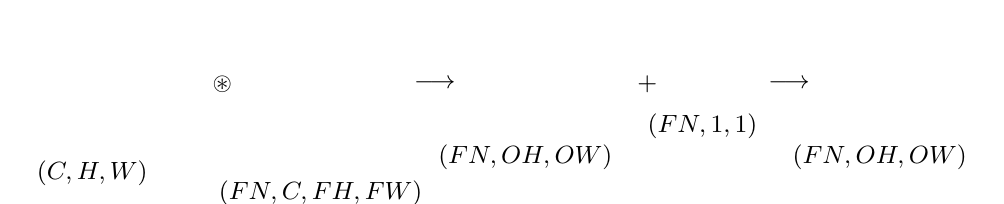
\begin{tikzpicture}
\cuboid{0}{0}{1.6}{1.6}{0.9}{blue}
\node[font=\small,below] at (0.8,-0.05) {$(C,H,W)$};
\node[font=\small] at (2.45,0.8) {$\circledast$};
\foreach \k in {3,2,1,0} {\cuboid{2.9+0.25*\k}{0.35-0.2*\k}{0.8}{0.8}{0.7}{blue}}
\node[font=\small,below] at (3.7,-0.3) {$(FN,C,FH,FW)$};
\node[font=\small] at (5.15,0.8) {$\longrightarrow$};
\cuboid{5.7}{0.2}{1.2}{1.2}{0.8}{orange}
\node[font=\small,below] at (6.3,0.15) {$(FN,OH,OW)$};
\node[font=\small] at (7.85,0.8) {$+$};
\cuboid{8.3}{0.65}{0.25}{0.25}{0.8}{orange}
\node[font=\small,below] at (8.55,0.55) {$(FN,1,1)$};
\node[font=\small] at (9.65,0.8) {$\longrightarrow$};
\cuboid{10.2}{0.2}{1.2}{1.2}{0.8}{orange}
\node[font=\small,below] at (10.8,0.15) {$(FN,OH,OW)$};
\end{tikzpicture}

\small 필터 $FN$개를 쓰는 합성곱 계층. 편향은 필터(출력 채널)마다 하나이다.
\end{center}

\begin{thinkbox}[왜 합성곱인가: 가중치 공유]
합성곱 계층에서는 \textbf{같은 필터를 이미지의 모든 위치에 적용}한다 (가중치 공유, weight sharing).
그래서 세로 획을 찾는 필터 하나가 이미지의 왼쪽 위에 있는 세로 획과 오른쪽 아래에 있는 세로 획을 똑같이 찾아낸다.
또 매개변수가 아주 적다. MNIST 이미지 $(1,28,28)$에서 $(30,24,24)$의 출력을 만든다고 하자.
\begin{itemize}[leftmargin=1.5em]
\item 완전연결 계층: $784\times(30\cdot24\cdot24)=784\times17280\approx1350$만 개의 가중치
\item 합성곱 계층 ($5\times5$ 필터 $30$개): $30\times1\times5\times5=750$개의 가중치와 $30$개의 편향
\end{itemize}
각 출력 원소는 입력의 $5\times5$ 영역만 본다 (\textbf{국소 연결}). 이 두 성질이 이미지의 구조에 잘 맞는다.
\end{thinkbox}

\subsection{배치 처리}\label{sec:convbatch}

완전연결 계층에서 미니배치로 데이터를 묶어 한 번에 처리했듯이, 합성곱 계층도 배치 처리를 한다.
각 계층을 흐르는 데이터에 차원을 하나 더 늘려 \textbf{4차원} (데이터 수, 채널, 높이, 너비) $=(N,C,H,W)$로 저장한다.
(지금까지 미니배치 크기를 $h$라 했지만, 이 장에서는 높이 $H$와 헷갈리지 않도록 $N$이라 쓴다.)

\begin{center}
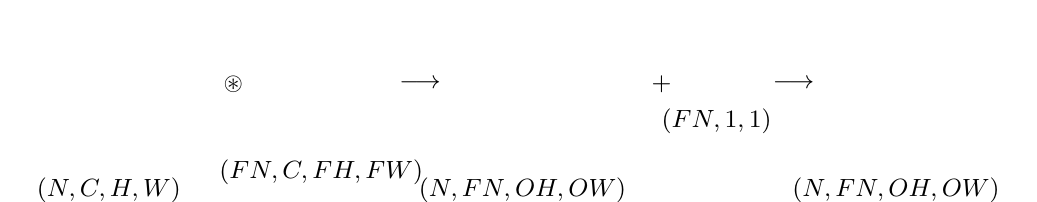
\begin{tikzpicture}[x=0.93cm,y=0.93cm]
\foreach \k in {2,1,0} {\cuboid{0.3*\k}{-0.25*\k}{1.4}{1.4}{0.8}{blue}}
\node[font=\small,below] at (0.95,-0.55) {$(N,C,H,W)$};
\node[font=\small] at (2.65,0.6) {$\circledast$};
\foreach \k in {3,2,1,0} {\cuboid{3.1+0.25*\k}{0.35-0.2*\k}{0.7}{0.7}{0.6}{blue}}
\node[font=\small,below] at (3.85,-0.3) {$(FN,C,FH,FW)$};
\node[font=\small] at (5.2,0.6) {$\longrightarrow$};
\foreach \k in {2,1,0} {\cuboid{5.8+0.3*\k}{-0.25*\k}{1.1}{1.1}{0.7}{orange}}
\node[font=\small,below] at (6.6,-0.55) {$(N,FN,OH,OW)$};
\node[font=\small] at (8.5,0.6) {$+$};
\cuboid{9.0}{0.45}{0.25}{0.25}{0.7}{orange}
\node[font=\small,below] at (9.25,0.4) {$(FN,1,1)$};
\node[font=\small] at (10.3,0.6) {$\longrightarrow$};
\foreach \k in {2,1,0} {\cuboid{10.9+0.3*\k}{-0.25*\k}{1.1}{1.1}{0.7}{orange}}
\node[font=\small,below] at (11.7,-0.55) {$(N,FN,OH,OW)$};
\end{tikzpicture}

\small 합성곱 연산의 배치 처리. $N$개의 데이터에 대한 합성곱을 한 번에 한다.
\end{center}

신경망에는 4차원 데이터가 하나 흐를 때마다 데이터 $N$개에 대한 합성곱 연산이 이루어진다.

% =================================================
\section{풀링 계층}\label{sec:pool}
% =================================================

\textbf{풀링(pooling)}은 세로, 가로 방향의 공간을 줄이는 연산이다.
아래는 $2\times2$ \textbf{최대 풀링(max pooling)}을 스트라이드 $2$로 하는 예이다.
$2\times2$ 영역마다 가장 큰 원소 하나를 꺼낸다.

\begin{center}
\begin{tikzpicture}
\fill[orange!30] (0,0) rectangle ({2*\cellsz},{-2*\cellsz});
\fill[blue!15] ({2*\cellsz},0) rectangle ({4*\cellsz},{-2*\cellsz});
\fill[green!20] (0,{-2*\cellsz}) rectangle ({2*\cellsz},{-4*\cellsz});
\fill[black!10] ({2*\cellsz},{-2*\cellsz}) rectangle ({4*\cellsz},{-4*\cellsz});
\numgrid{0}{0}{4}{1,2,1,0,0,1,2,3,3,0,1,2,2,4,0,1}
\draw[very thick] (0,0) rectangle ({4*\cellsz},{-4*\cellsz});
\draw[very thick] ({2*\cellsz},0) -- ({2*\cellsz},{-4*\cellsz});
\draw[very thick] (0,{-2*\cellsz}) -- ({4*\cellsz},{-2*\cellsz});
\node[font=\Large] at (3,-1) {$\longrightarrow$};
\fill[orange!30] (3.8,-0.5) rectangle ++(\cellsz,-\cellsz);
\fill[blue!15] ({3.8+\cellsz},-0.5) rectangle ++(\cellsz,-\cellsz);
\fill[green!20] (3.8,{-0.5-\cellsz}) rectangle ++(\cellsz,-\cellsz);
\fill[black!10] ({3.8+\cellsz},{-0.5-\cellsz}) rectangle ++(\cellsz,-\cellsz);
\numgrid{3.8}{-0.5}{2}{2,3,4,2}
\node[font=\small,below] at (1,-2.1) {입력 $(4,4)$};
\node[font=\small,below] at (4.3,-2.1) {출력 $(2,2)$};
\end{tikzpicture}
\end{center}

풀링의 윈도우 크기와 스트라이드는 보통 같은 값으로 한다 (윈도우 $3\times3$이면 스트라이드 $3$).
최대 풀링 외에 영역의 평균을 내는 \textbf{평균 풀링(average pooling)}도 있지만,
이미지 인식에서는 주로 최대 풀링을 쓴다. 이 노트에서 풀링이라 하면 최대 풀링을 뜻한다.

\begin{keybox}[풀링 계층의 특징]
\begin{itemize}[leftmargin=1.5em]
\item \textbf{학습해야 할 매개변수가 없다.} 영역에서 최댓값(또는 평균)을 취하는 명확한 처리일 뿐이다.
\item \textbf{채널 수가 변하지 않는다.} 채널마다 독립적으로 계산한다: $(N,C,H,W)\to(N,C,OH,OW)$.
\item \textbf{입력의 작은 변화에 영향을 적게 받는다(robust).}
입력이 한두 칸 이동해도 영역 안의 최댓값은 그대로인 경우가 많다.
\end{itemize}
\end{keybox}
\begin{lstlisting}
pool = Pooling(2, 2)                                    # max pooling, 2x2 window, stride 2
\end{lstlisting}
\begin{lstlisting}[language={},numbers=none]
2x2 max pooling:
 [[2. 3.]
 [4. 2.]]
\end{lstlisting}

% =================================================
\section{합성곱 / 풀링 계층 구현하기}\label{sec:impl}
% =================================================

지금까지 그래 왔듯이 합성곱 계층과 풀링 계층도 \texttt{forward}와 \texttt{backward}를 가진 클래스로 구현한다.
코드는 \texttt{code/conv\_layers.py}에 있고, Affine, ReLU, Softmax 계층은 지난 시간의 \texttt{layers.py}를 그대로 쓴다.

\begin{center}
\begin{tabular}{@{}p{0.3\textwidth}p{0.64\textwidth}@{}}
\toprule
파일 & 내용 \\
\midrule
\texttt{conv\_layers.py} & \texttt{im2col}, \texttt{col2im}, \texttt{Convolution}, \texttt{Pooling}, \texttt{Flatten}, \texttt{SimpleConvNet} \\
\texttt{layers.py}, \texttt{optimizers.py}, \texttt{mnist\_data.py} & 지난 시간의 모듈 (그대로 복사) \\[2pt]
\texttt{cat\_parts.py} & 도입부의 고양이 사진과 부분 그림 \\
\texttt{classic\_filters.py} & 사람이 설계한 필터 (평균, Sobel, Laplacian 등)를 흑백 사진에 적용 \\
\texttt{conv\_basics.py} & 이 노트의 예제, im2col 확인과 속도 비교, gradient 확인 \\
\texttt{mnist\_cnn.py} & SimpleConvNet으로 MNIST 학습, 필터와 특징 맵 시각화 \\
\texttt{mnist\_cnn\_torch.py} & 같은 network를 PyTorch로 \\
\bottomrule
\end{tabular}
\end{center}

\subsection{4차원 배열}\label{sec:4d}

CNN에서 계층 사이를 흐르는 데이터는 4차원 배열 $(N,C,H,W)$이다.
예를 들어 높이 $28$, 너비 $28$, 채널 $1$인 데이터가 $10$개라면 shape은 $(10,1,28,28)$이다.
\begin{lstlisting}[language={},numbers=none]
>>> x = np.random.rand(10, 1, 28, 28)
>>> x[0].shape         # the first image: (1, 28, 28)
>>> x[0, 0].shape      # its first channel: (28, 28)
\end{lstlisting}
지금까지 MNIST를 $(N,784)$로 다루었지만, CNN에서는 \texttt{reshape}으로 모양을 되살려 입력한다 (\texttt{mnist\_cnn.py}).
\begin{lstlisting}
x_train, t_train, x_val, t_val, x_test, t_test = load_mnist_split()
# a CNN keeps the SHAPE of the image: (N, 784) -> (N, 1, 28, 28) = (images, channels, height, width)
x_train = x_train.reshape(-1, 1, 28, 28)
\end{lstlisting}

\subsection{im2col로 데이터 전개하기}\label{sec:im2col}

합성곱을 \ref{sec:convop}절의 \texttt{conv2d\_naive}처럼 반복문으로 구현하면,
데이터 $N$개, 필터 $FN$개, 출력의 모든 위치 $OH\times OW$에 대하여 \texttt{for} 문이 겹겹이 필요하다.
numpy에서 \texttt{for} 문은 느리다. 그래서 \textbf{im2col}(image to column)이라는 함수로
입력 데이터를 필터를 적용하기 좋게 \textbf{2차원 행렬로 펼친다}.

\begin{keybox}[im2col의 아이디어]
필터가 방문하는 위치 하나마다, 그 위치의 입력 영역 $(C,FH,FW)$을 \textbf{한 행}으로 펼친다.
\begin{itemize}[leftmargin=1.5em]
\item 입력 $(N,C,H,W)$ $\xrightarrow{\text{im2col}}$ 행렬 $(N\cdot OH\cdot OW,\ C\cdot FH\cdot FW)$
\item 필터 $(FN,C,FH,FW)$ $\xrightarrow{\text{reshape}}$ 필터 하나를 \textbf{한 열}로: $(C\cdot FH\cdot FW,\ FN)$
\item 합성곱 $=$ 두 행렬의 곱 $+$ 편향: $(N\cdot OH\cdot OW,\ FN)$ $\xrightarrow{\text{reshape}}$ $(N,FN,OH,OW)$
\end{itemize}
\end{keybox}

\begin{center}
\begin{tikzpicture}[>=Latex]
% input with two windows
\cuboid{0}{0}{1.8}{1.8}{0.6}{blue}
\filldraw[fill=orange!50,draw=orange!80!black,thick] (0,1.8) rectangle ++(0.9,-0.9);
\filldraw[fill=green!40,draw=green!50!black,thick] (0.45,1.8) rectangle ++(0.9,-0.9);
\node[font=\scriptsize] at (0.3,1.1) {\ding{172}};
\node[font=\scriptsize] at (1.2,1.1) {\ding{173}};
\node[font=\small,below] at (0.9,-0.05) {입력 $(C,H,W)$};
\draw[->,thick] (2.5,0.8) -- node[above,font=\small] {im2col} (3.5,0.8);
% the column matrix: one row per filter position
\fill[orange!50] (3.7,2.0) rectangle (5.7,1.75);
\fill[green!40] (3.7,1.75) rectangle (5.7,1.5);
\draw[thick] (3.7,2.0) rectangle (5.7,-0.4);
\node[font=\scriptsize,anchor=east] at (3.65,1.875) {\ding{172}};
\node[font=\scriptsize,anchor=east] at (3.65,1.625) {\ding{173}};
\node[font=\small] at (4.7,0.6) {$\vdots$};
\node[font=\small,below,align=center] at (4.7,-0.45) {$(OH\cdot OW,$\\$C\cdot FH\cdot FW)$};
% the filters: one column per filter
\node[font=\Large] at (6.05,0.8) {$\cdot$};
\fill[blue!25] (6.4,2.0) rectangle (6.7,-0.4);
\fill[blue!45] (6.7,2.0) rectangle (7.0,-0.4);
\draw[thick] (6.4,2.0) rectangle (7.6,-0.4);
\node[font=\small,below,align=center] at (7.0,-0.45) {$(C\cdot FH\cdot FW,$\\$FN)$};
\node[font=\Large] at (8.1,0.8) {$=$};
\fill[orange!50] (8.6,2.0) rectangle (9.8,1.75);
\fill[green!40] (8.6,1.75) rectangle (9.8,1.5);
\draw[thick] (8.6,2.0) rectangle (9.8,-0.4);
\node[font=\small,below,align=center] at (9.2,-0.45) {$(OH\cdot OW,$\\$FN)$};
\draw[->,thick] (10.0,0.8) -- node[above,font=\small] {reshape} (11.2,0.8);
\cuboid{11.4}{0.2}{1.1}{1.1}{0.6}{orange}
\node[font=\small,below] at (11.95,0.15) {$(FN,OH,OW)$};
\end{tikzpicture}

\small im2col을 이용한 합성곱 (데이터 하나의 경우). 필터의 위치 \ding{172}, \ding{173}, $\ldots$이 행렬의 각 행이 된다.
\end{center}

이렇게 하면 합성곱 계층의 순전파는 \textbf{Affine 계층과 똑같은} 행렬곱 $A=\text{col}\cdot W_{\text{col}}+B$가 된다.
행렬곱은 numpy가 최적화된 선형대수 라이브러리(BLAS)로 계산하므로 매우 빠르다.
\begin{lstlisting}
def im2col(X, FH, FW, stride=1, pad=0):
    """(N, C, H, W) -> (N*OH*OW, C*FH*FW): ONE ROW for every place the filter visits"""
    N, C, H, W = X.shape
    OH, OW = output_size(H, FH, stride, pad), output_size(W, FW, stride, pad)
    Xp = np.pad(X, [(0, 0), (0, 0), (pad, pad), (pad, pad)])    # zero padding
    col = np.zeros((N, C, FH, FW, OH, OW))
    for i in range(FH):                   # loop over the FILTER, not the image
        for j in range(FW):
            col[:, :, i, j, :, :] = Xp[:, :, i:i + stride * OH:stride, j:j + stride * OW:stride]
    return col.transpose(0, 4, 5, 1, 2, 3).reshape(N * OH * OW, -1)
\end{lstlisting}
반복문은 이미지 전체가 아니라 \textbf{필터의 크기} ($FH\times FW$, 예: $5\times5=25$번)만큼만 돈다.
\texttt{(i, j)} 번째 반복에서는 ``필터의 $(i,j)$ 원소와 곱해질 입력의 값들''을 모든 출력 위치에 대해 한꺼번에 잘라 온다.
마지막 \texttt{transpose}와 \texttt{reshape}으로 출력 위치마다 한 행이 되도록 정리한다.
\begin{lstlisting}
x1 = np.random.rand(1, 3, 7, 7)                         # 1 image, 3 channels, 7x7
print("im2col of (1, 3, 7, 7) with a 5x5 filter:", im2col(x1, 5, 5).shape)
x2 = np.random.rand(10, 3, 7, 7)                        # 10 images
print("im2col of (10, 3, 7, 7) with a 5x5 filter:", im2col(x2, 5, 5).shape)
\end{lstlisting}
\begin{lstlisting}[language={},numbers=none]
im2col of (1, 3, 7, 7) with a 5x5 filter: (9, 75)
im2col of (10, 3, 7, 7) with a 5x5 filter: (90, 75)
\end{lstlisting}
$7\times7$ 입력에 $5\times5$ 필터를 적용하면 출력은 $3\times3=9$개의 위치이고,
각 위치의 입력 영역은 $3\times5\times5=75$개의 값이다. 데이터가 $10$개이면 행이 $90$개가 된다.

\paragraph{얼마나 빠를까?}
MNIST 크기의 미니배치 $(100,1,28,28)$에 $5\times5$ 필터 $30$개를 적용하는 합성곱을,
네 겹의 반복문과 im2col로 각각 계산해 비교한다.
\begin{lstlisting}
def conv_loops(X, W, B):
    """(N, C, H, W) with FN filters (FN, C, FH, FW): every image, every filter, every position"""
    N, C, H, Wd = X.shape
    FN, _, FH, FW = W.shape
    OH, OW = H - FH + 1, Wd - FW + 1
    Y = np.zeros((N, FN, OH, OW))
    for n in range(N):
        for k in range(FN):
            for i in range(OH):
                for j in range(OW):
                    Y[n, k, i, j] = np.sum(X[n, :, i:i + FH, j:j + FW] * W[k]) + B[k]
    return Y
\end{lstlisting}
\begin{lstlisting}[language={},numbers=none]
output shape (100, 30, 24, 24), max |difference| = 5.3e-15
loops 5.74 s,  im2col 0.057 s  (101 times faster)
\end{lstlisting}
결과는 같고 (차이 $10^{-15}$), im2col이 약 $100$배 빠르다.
반복문으로는 미니배치 하나에 $6$초가 걸리므로, $550$개의 미니배치로 이루어진 한 epoch에 거의 $1$시간이 걸린다.

\begin{remarkbox}[im2col의 대가: 메모리]
필터가 겹쳐서 이동하면 입력의 같은 값이 im2col 행렬의 여러 행에 중복해서 들어간다.
$(100,1,28,28)$ 입력 ($78400$개의 값)이 $5\times5$ 필터로 전개되면
$(100\cdot24\cdot24,\ 25)=(57600,25)$, 즉 $144$만 개의 값이 된다. 약 $18$배이다.
메모리를 더 쓰는 대신 속도를 얻는 것이다.
그래서 \texttt{SimpleConvNet}의 \texttt{accuracy}는 $10000$장을 한꺼번에 넣지 않고 $1000$장씩 나누어 계산한다.
GPU용 라이브러리(cuDNN 등)는 im2col 외에도 FFT, Winograd 같은 여러 방법을 상황에 따라 골라 쓴다.
\end{remarkbox}

\subsection{합성곱 계층 구현하기}\label{sec:convlayer}

im2col을 쓰면 합성곱 계층의 순전파는 ``im2col $\to$ Affine $\to$ reshape''이다.
\begin{lstlisting}
class Convolution:
    """Convolution of (N, C, H, W) with FN filters (FN, C, FH, FW) -> (N, FN, OH, OW).
       With im2col: ONE matrix product, i.e. an Affine layer at every filter position."""
    def __init__(self, W, B, stride=1, pad=0):
        self.W = W                  # (FN, C, FH, FW)
        self.B = B                  # (FN,): one bias per filter
        self.stride = stride
        self.pad = pad
        self.dW = None
        self.dB = None

    def forward(self, X):
        FN, C, FH, FW = self.W.shape
        N, _, H, W = X.shape
        OH = output_size(H, FH, self.stride, self.pad)
        OW = output_size(W, FW, self.stride, self.pad)
        self.X_shape = X.shape
        self.col = im2col(X, FH, FW, self.stride, self.pad)     # (N*OH*OW, C*FH*FW)
        self.W_col = self.W.reshape(FN, -1).T                    # one filter per COLUMN
        A = self.col @ self.W_col + self.B                       # (N*OH*OW, FN)
        return A.reshape(N, OH, OW, FN).transpose(0, 3, 1, 2)    # (N, FN, OH, OW)
\end{lstlisting}
\texttt{A}의 각 행은 (데이터, 출력 위치) 하나, 각 열은 필터(출력 채널) 하나이다.
그래서 \texttt{reshape(N, OH, OW, FN)}으로 나눈 뒤, 채널 축을 두 번째로 옮겨 $(N,FN,OH,OW)$를 만든다.
출력 크기는 \ref{sec:stride}절의 식을 그대로 함수로 만든 것이다.
\begin{lstlisting}
def output_size(H, FH, stride=1, pad=0):
    """height (or width) of the output: OH = (H + 2P - FH) / S + 1"""
    return (H + 2 * pad - FH) // stride + 1
\end{lstlisting}

\paragraph{합성곱 계층의 역전파.}
순전파가 세 단계로 나뉘었으므로, 변수 노드 기준의 계산 그래프로 그리면 다음과 같다.

\begin{center}
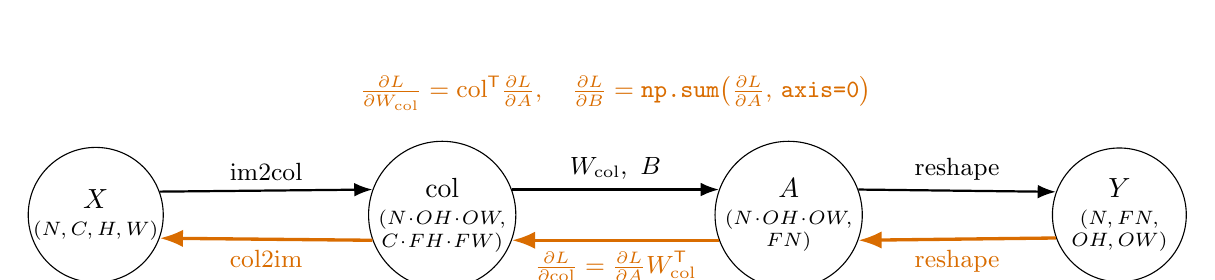
\begin{tikzpicture}[>=Latex,
  var/.style={draw,circle,minimum size=17mm,align=center,inner sep=0pt},
  bw/.style={<-,very thick,orange!85!black},
  bl/.style={orange!85!black,font=\small,align=center}]
\node[var] (X) at (0,0) {$X$\\[-2pt]{\scriptsize $(N,C,H,W)$}};
\node[var] (col) at (4.4,0) {col\\[-2pt]{\scriptsize $(N\!\cdot\!OH\!\cdot\!OW,$}\\[-4pt]{\scriptsize $C\!\cdot\!FH\!\cdot\!FW)$}};
\node[var] (A) at (8.8,0) {$A$\\[-2pt]{\scriptsize $(N\!\cdot\!OH\!\cdot\!OW,$}\\[-4pt]{\scriptsize $FN)$}};
\node[var] (Y) at (13.0,0) {$Y$\\[-2pt]{\scriptsize $(N,FN,$}\\[-4pt]{\scriptsize $OH,OW)$}};
\draw[->,thick] (X.20) -- node[above,font=\small] {im2col} (col.160);
\draw[->,thick] (col.20) -- node[above,font=\small] {$W_{\text{col}},\ B$} (A.160);
\draw[->,thick] (A.20) -- node[above,font=\small] {reshape} (Y.160);
\draw[bw] (X.-20) -- node[below,bl] {col2im} (col.-160);
\draw[bw] (col.-20) -- node[below,bl] {$\pd{L}{\text{col}}=\pd{L}{A}W_{\text{col}}\T$} (A.-160);
\draw[bw] (A.-20) -- node[below,bl] {reshape} (Y.-160);
\node[bl] at (6.6,1.55) {$\pd{L}{W_{\text{col}}}=\text{col}\T\pd{L}{A},\quad \pd{L}{B}=\texttt{np.sum}\bigl(\pd{L}{A},\,\texttt{axis=0}\bigr)$};
\end{tikzpicture}

\small 합성곱 계층의 계산 그래프. 가운데는 지난 시간의 Affine 계층 그대로이다.
\end{center}

\begin{itemize}[leftmargin=1.8em]
\item \textbf{reshape의 역전파}는 gradient의 모양을 원래대로 되돌리는 것뿐이다 (값은 그대로 전달).
\item \textbf{가운데는 Affine 계층}이다. 지난 시간에 유도한
$\pd{L}{W}=X\T\pd{L}{A}$, $\pd{L}{B}=\sum_{\text{행}}\pd{L}{A}$, $\pd{L}{X}=\pd{L}{A}W\T$를 그대로 쓴다.
\item \textbf{im2col의 역전파}는 \textbf{col2im}이다. im2col에서 입력의 한 값이 col의 여러 행에 복사되었으므로
(필터 위치가 겹치는 곳), 역전파에서는 그 값으로 돌아오는 gradient를 \textbf{모두 더해야} 한다.
한 변수에서 화살표가 여러 개 나가면 gradient를 더한다는 다변수 연쇄법칙(배치 정규화에서 보았다)과 같은 원리이다.
\end{itemize}

\begin{lstlisting}
    def backward(self, dA):
        FN, C, FH, FW = self.W.shape
        dA = dA.transpose(0, 2, 3, 1).reshape(-1, FN)            # (N*OH*OW, FN)
        self.dB = np.sum(dA, axis=0)                             # the Affine rules
        self.dW = (self.col.T @ dA).T.reshape(FN, C, FH, FW)
        dcol = dA @ self.W_col.T                                 # (N*OH*OW, C*FH*FW)
        return col2im(dcol, self.X_shape, FH, FW, self.stride, self.pad)
\end{lstlisting}
\begin{lstlisting}
def col2im(col, X_shape, FH, FW, stride=1, pad=0):
    """the reverse of im2col: ADD every row back where it came from"""
    N, C, H, W = X_shape
    OH, OW = output_size(H, FH, stride, pad), output_size(W, FW, stride, pad)
    col = col.reshape(N, OH, OW, C, FH, FW).transpose(0, 3, 4, 5, 1, 2)
    Xp = np.zeros((N, C, H + 2 * pad, W + 2 * pad))
    for i in range(FH):
        for j in range(FW):
            Xp[:, :, i:i + stride * OH:stride, j:j + stride * OW:stride] += col[:, :, i, j, :, :]
    return Xp[:, :, pad:pad + H, pad:pad + W]     # remove the padding
\end{lstlisting}
im2col에서 \texttt{=}로 잘라 온 자리에, col2im에서는 \texttt{+=}로 더해 넣는다는 것만 다르다.

\subsection{풀링 계층 구현하기}\label{sec:poollayer}

풀링 계층도 im2col로 입력을 전개한다. 다만 풀링은 \textbf{채널마다 독립적}이므로,
전개한 뒤 한 행이 ``한 채널의 한 윈도우''가 되도록 다시 \texttt{reshape}하고, 행마다 최댓값을 구한다.

\begin{center}
\begin{tikzpicture}
\fill[orange!30] (0,0) rectangle ({2*\cellsz},{-2*\cellsz});
\fill[blue!15] ({2*\cellsz},0) rectangle ({4*\cellsz},{-2*\cellsz});
\fill[green!20] (0,{-2*\cellsz}) rectangle ({2*\cellsz},{-4*\cellsz});
\fill[black!10] ({2*\cellsz},{-2*\cellsz}) rectangle ({4*\cellsz},{-4*\cellsz});
\numgrid{0}{0}{4}{1,2,1,0,0,1,2,3,3,0,1,2,2,4,0,1}
\node[font=\small] at (2.9,-1) {$\xrightarrow{\text{전개}}$};
\fill[orange!30] (3.6,0) rectangle ++({4*\cellsz},-\cellsz);
\fill[blue!15] (3.6,-\cellsz) rectangle ++({4*\cellsz},-\cellsz);
\fill[green!20] (3.6,{-2*\cellsz}) rectangle ++({4*\cellsz},-\cellsz);
\fill[black!10] (3.6,{-3*\cellsz}) rectangle ++({4*\cellsz},-\cellsz);
\numgrid{3.6}{0}{4}{1,2,0,1,1,0,2,3,3,0,2,4,1,2,0,1}
\node[font=\small] at (6.4,-1) {$\xrightarrow{\text{max}}$};
\numgrid{7.2}{0}{1}{2,3,4,2}
\node[font=\small] at (8.4,-1) {$\xrightarrow{\text{reshape}}$};
\numgrid{9.3}{-0.5}{2}{2,3,4,2}
\end{tikzpicture}

\small 풀링 계층의 구현: 윈도우마다 한 행으로 전개하고, 행마다 최댓값을 구한 뒤 모양을 되돌린다.
\end{center}

\begin{lstlisting}
    def forward(self, X):
        N, C, H, W = X.shape
        OH = output_size(H, self.PH, self.stride, self.pad)
        OW = output_size(W, self.PW, self.stride, self.pad)
        col = im2col(X, self.PH, self.PW, self.stride, self.pad)
        col = col.reshape(-1, self.PH * self.PW)           # one window per row
        self.argmax = np.argmax(col, axis=1)               # where the maximum was
        self.X_shape = X.shape
        Y = np.max(col, axis=1)
        return Y.reshape(N, OH, OW, C).transpose(0, 3, 1, 2)   # (N, C, OH, OW)
\end{lstlisting}

\paragraph{풀링 계층의 역전파.}
$y=\max(x_1,x_2,x_3,x_4)$에서 최댓값이 $x_k$이면 $\pd{y}{x_k}=1$이고 나머지는 $0$이다.
즉 최댓값이었던 원소에만 gradient를 그대로 전달하고, 나머지에는 $0$을 보낸다.
ReLU에서 \texttt{mask}로 통과한 원소에만 gradient를 보낸 것과 같다.
순전파에서 최댓값의 위치(\texttt{argmax})를 기억해 두는 이유이다.
(최댓값이 여러 개로 같으면 미분이 하나로 정해지지 않는다. 이 구현은 \texttt{np.argmax}가 고른 첫 위치로 보낸다.)
\begin{lstlisting}
    def backward(self, dY):
        dY = dY.transpose(0, 2, 3, 1).ravel()               # the same order as col
        dcol = np.zeros((dY.size, self.PH * self.PW))
        dcol[np.arange(dY.size), self.argmax] = dY          # only the max gets it
        dcol = dcol.reshape(-1, self.X_shape[1] * self.PH * self.PW)
        return col2im(dcol, self.X_shape, self.PH, self.PW, self.stride, self.pad)
\end{lstlisting}

\subsection{Flatten 계층}\label{sec:flatten}

합성곱과 풀링을 거친 4차원 데이터를 Affine 계층에 넣으려면 데이터마다 한 줄로 펼쳐야 한다.
이것을 계층 하나로 만들어 둔다 (PyTorch의 \texttt{nn.Flatten}). 역전파는 모양을 되돌리는 것뿐이다.
\begin{lstlisting}
class Flatten:
    """(N, C, H, W) -> (N, C*H*W) before an Affine layer (nn.Flatten in PyTorch)"""
    def forward(self, X):
        self.X_shape = X.shape
        return X.reshape(X.shape[0], -1)

    def backward(self, dY):
        return dY.reshape(self.X_shape)
\end{lstlisting}

% =================================================
\section{CNN 구현하기}\label{sec:simplecnn}
% =================================================

합성곱 계층과 풀링 계층을 조합하여 손글씨 숫자를 인식하는 CNN (\texttt{SimpleConvNet})을 만든다.

\begin{center}
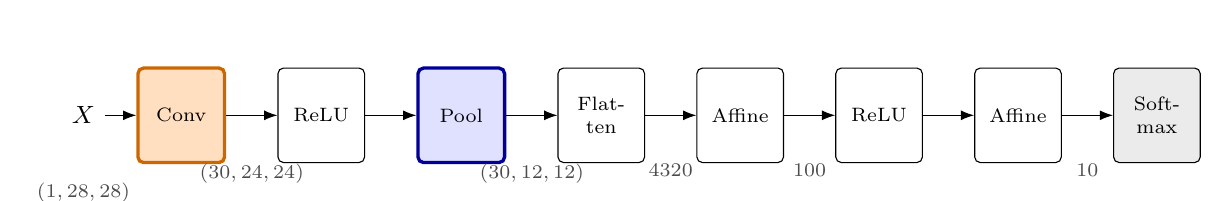
\begin{tikzpicture}[>=Latex,
  lay/.style={draw,rounded corners=2pt,minimum width=11mm,minimum height=12mm,
              font=\scriptsize,align=center,inner sep=1pt},
  cv/.style={lay,fill=orange!25,draw=orange!80!black,very thick},
  pl/.style={lay,fill=blue!12,draw=blue!60!black,very thick},
  sh/.style={font=\scriptsize,align=center,text=black!70},
  node distance=6.5mm]
\node[font=\small] (in) {$X$};
\node[cv,right=4mm of in] (c1) {Conv};
\node[lay,right=of c1] (r1) {ReLU};
\node[pl,right=of r1] (p1) {Pool};
\node[lay,right=of p1] (f1) {Flat-\\ten};
\node[lay,right=of f1] (a1) {Affine};
\node[lay,right=of a1] (r2) {ReLU};
\node[lay,right=of r2] (a2) {Affine};
\node[lay,right=of a2,fill=black!8] (sm) {Soft-\\max};
\draw[->] (in) -- (c1);
\draw[->] (c1) -- node[sh,below=5mm] {$(30,24,24)$} (r1);
\draw[->] (r1) -- (p1);
\draw[->] (p1) -- node[sh,below=5mm] {$(30,12,12)$} (f1);
\draw[->] (f1) -- node[sh,below=5mm] {$4320$} (a1);
\draw[->] (a1) -- node[sh,below=5mm] {$100$} (r2);
\draw[->] (r2) -- (a2);
\draw[->] (a2) -- node[sh,below=5mm] {$10$} (sm);
\node[sh,below=5mm] at (in.south) {$(1,28,28)$};
\end{tikzpicture}

\small SimpleConvNet의 구조와 각 계층을 지난 뒤 데이터 하나의 shape
\end{center}

\begin{center}
{\small
\begin{tabular}{@{}llcr@{}}
\toprule
계층 & 설정 & 출력 shape & 매개변수 수 \\
\midrule
입력 & & $(1,28,28)$ & \\
Conv & $5\times5$ 필터 $30$개 & $(30,24,24)$ & $30\cdot1\cdot5\cdot5+30=780$ \\
ReLU & & $(30,24,24)$ & \\
Pooling & $2\times2$ 최대 풀링 & $(30,12,12)$ & \\
Flatten & & $4320$ & \\
Affine & & $100$ & $4320\cdot100+100=432100$ \\
ReLU & & $100$ & \\
Affine & & $10$ & $100\cdot10+10=1010$ \\
\midrule
합계 & & & $433890$ \\
\bottomrule
\end{tabular}}

(합성곱은 스트라이드 $1$, 패딩 $0$, 풀링은 스트라이드 $2$이다. 출력 shape은 데이터 하나의 것이다.)
\end{center}

합성곱 계층의 매개변수는 $780$개뿐이고, 매개변수의 $99.6\%$는 첫 번째 Affine 계층에 있다.
합성곱 계층이 가중치를 공유하기 때문이다 (\ref{sec:blocks}절).

\texttt{SimpleConvNet}은 지난 시간의 \texttt{MultiLayerNet}과 같은 방식으로 만든다.
매개변수를 \texttt{params} 딕셔너리에 두고, 같은 배열을 계층에도 넘겨주어
optimizer가 \texttt{params}를 갱신하면 계층의 가중치도 바뀌게 한다.
초깃값의 표준편차는 \texttt{weight\_init\_std}로 정한다. \texttt{"he"}이면 He 초깃값이고
(합성곱 필터 하나가 보는 입력의 수는 $C\cdot FH\cdot FW=25$개이므로 표준편차 $\sqrt{2/25}$), 숫자이면 그 값을 표준편차로 쓴다.
\begin{lstlisting}
class SimpleConvNet:
    """Conv -> ReLU -> Pool -> Flatten -> Affine -> ReLU -> Affine -> Softmax"""
    def __init__(self, input_shape=(1, 28, 28), filter_num=30, filter_size=5,
                 hidden_size=100, output_size=10, weight_init_std="he"):
        C, H, W = input_shape
        conv_out = H - filter_size + 1                     # 28 - 5 + 1 = 24
        pool_out = conv_out // 2                           # 2x2 max pooling: 12
        flat = filter_num * pool_out * pool_out            # 30 * 12 * 12 = 4320
        n_in = C * filter_size * filter_size               # 25 inputs per filter
        def std(n):                                        # "he": sqrt(2 / n_in), or a fixed number such as 0.01
            return np.sqrt(2.0 / n) if weight_init_std == "he" else weight_init_std
        self.params = {
            "W1": std(n_in) * np.random.randn(filter_num, C, filter_size, filter_size),
            "B1": np.zeros(filter_num),
            "W2": std(flat) * np.random.randn(flat, hidden_size),
            "B2": np.zeros((1, hidden_size)),
            "W3": std(hidden_size) * np.random.randn(hidden_size, output_size),
            "B3": np.zeros((1, output_size)),
        }
        self.layers = [
            Convolution(self.params["W1"], self.params["B1"]),
            Relu(),
            Pooling(2, 2),
            Flatten(),
            Affine(self.params["W2"], self.params["B2"]),
            Relu(),
            Affine(self.params["W3"], self.params["B3"]),
        ]
        self.last = SoftmaxWithCrossEntropy()
\end{lstlisting}
순전파, 손실, 역전파는 \texttt{MultiLayerNet}과 똑같다.
계층이 모두 같은 \texttt{forward}, \texttt{backward} 형식을 따르기 때문에,
새로운 계층이 들어와도 network 코드는 바뀌지 않는다. 이것이 계층 단위로 구현하는 장점이다.
\begin{lstlisting}
    def backward(self):                       # call right after loss()
        d = self.last.backward()
        for layer in reversed(self.layers):   # layer after layer
            d = layer.backward(d)
        grads, k = {}, 0
        for layer in self.layers:
            if isinstance(layer, (Convolution, Affine)):
                k += 1
                grads[f"W{k}"], grads[f"B{k}"] = layer.dW, layer.dB
        return grads
\end{lstlisting}

\paragraph{gradient 확인.}
작은 \texttt{SimpleConvNet} (입력 $(2,8,8)$, $3\times3$ 필터 $3$개)으로 역전파와 수치미분을 비교한다
(\texttt{conv\_basics.py}의 (3)).
\begin{lstlisting}
np.random.seed(1)
small = SimpleConvNet(input_shape=(2, 8, 8), filter_num=3, filter_size=3, hidden_size=5, output_size=4)
X_small = np.random.randn(5, 2, 8, 8)                   # 5 images, 2 channels, 8x8
T_small = np.eye(4)[np.random.randint(0, 4, size=5)]
small.loss(X_small, T_small)
grads = small.backward()
\end{lstlisting}
\begin{lstlisting}[language={},numbers=none]
W1: shape (3, 2, 3, 3)    max |backprop - numerical| = 1.15e-09
B1: shape (3,)            max |backprop - numerical| = 1.22e-09
W2: shape (27, 5)         max |backprop - numerical| = 1.42e-09
B2: shape (1, 5)          max |backprop - numerical| = 6.68e-10
W3: shape (5, 4)          max |backprop - numerical| = 1.03e-09
B3: shape (1, 4)          max |backprop - numerical| = 3.82e-10
\end{lstlisting}
합성곱, 풀링, Flatten을 지나는 역전파가 모두 올바르다.

\paragraph{MNIST로 학습하기.}
\texttt{mnist\_cnn.py}에서 \texttt{SimpleConvNet}을 Adam (학습률 $0.001$, 미니배치 $100$)으로 $10$ epoch 학습시킨다.
초깃값은 표준편차 $0.01$의 작은 값으로 시작한다. 그래야 학습으로 생긴 필터의 무늬가 잘 드러난다 (\ref{sec:filters}절).
비교를 위해 지난 시간의 다층 퍼셉트론(MLP, $784\to100\to10$, He 초깃값)도 같은 조건으로 학습시킨다.
\begin{lstlisting}
np.random.seed(1)
cnn = SimpleConvNet(input_shape=(1, 28, 28), filter_num=30, filter_size=5,
                    hidden_size=100, output_size=10,
                    weight_init_std=0.01)             # start small
print("SimpleConvNet parameters:", cnn.num_params())
W1_before = cnn.params["W1"].copy()                   # the filters before training
cnn_result = train(cnn)
\end{lstlisting}

\IfFileExists{figures/cnn_mnist.png}{%
\begin{center}
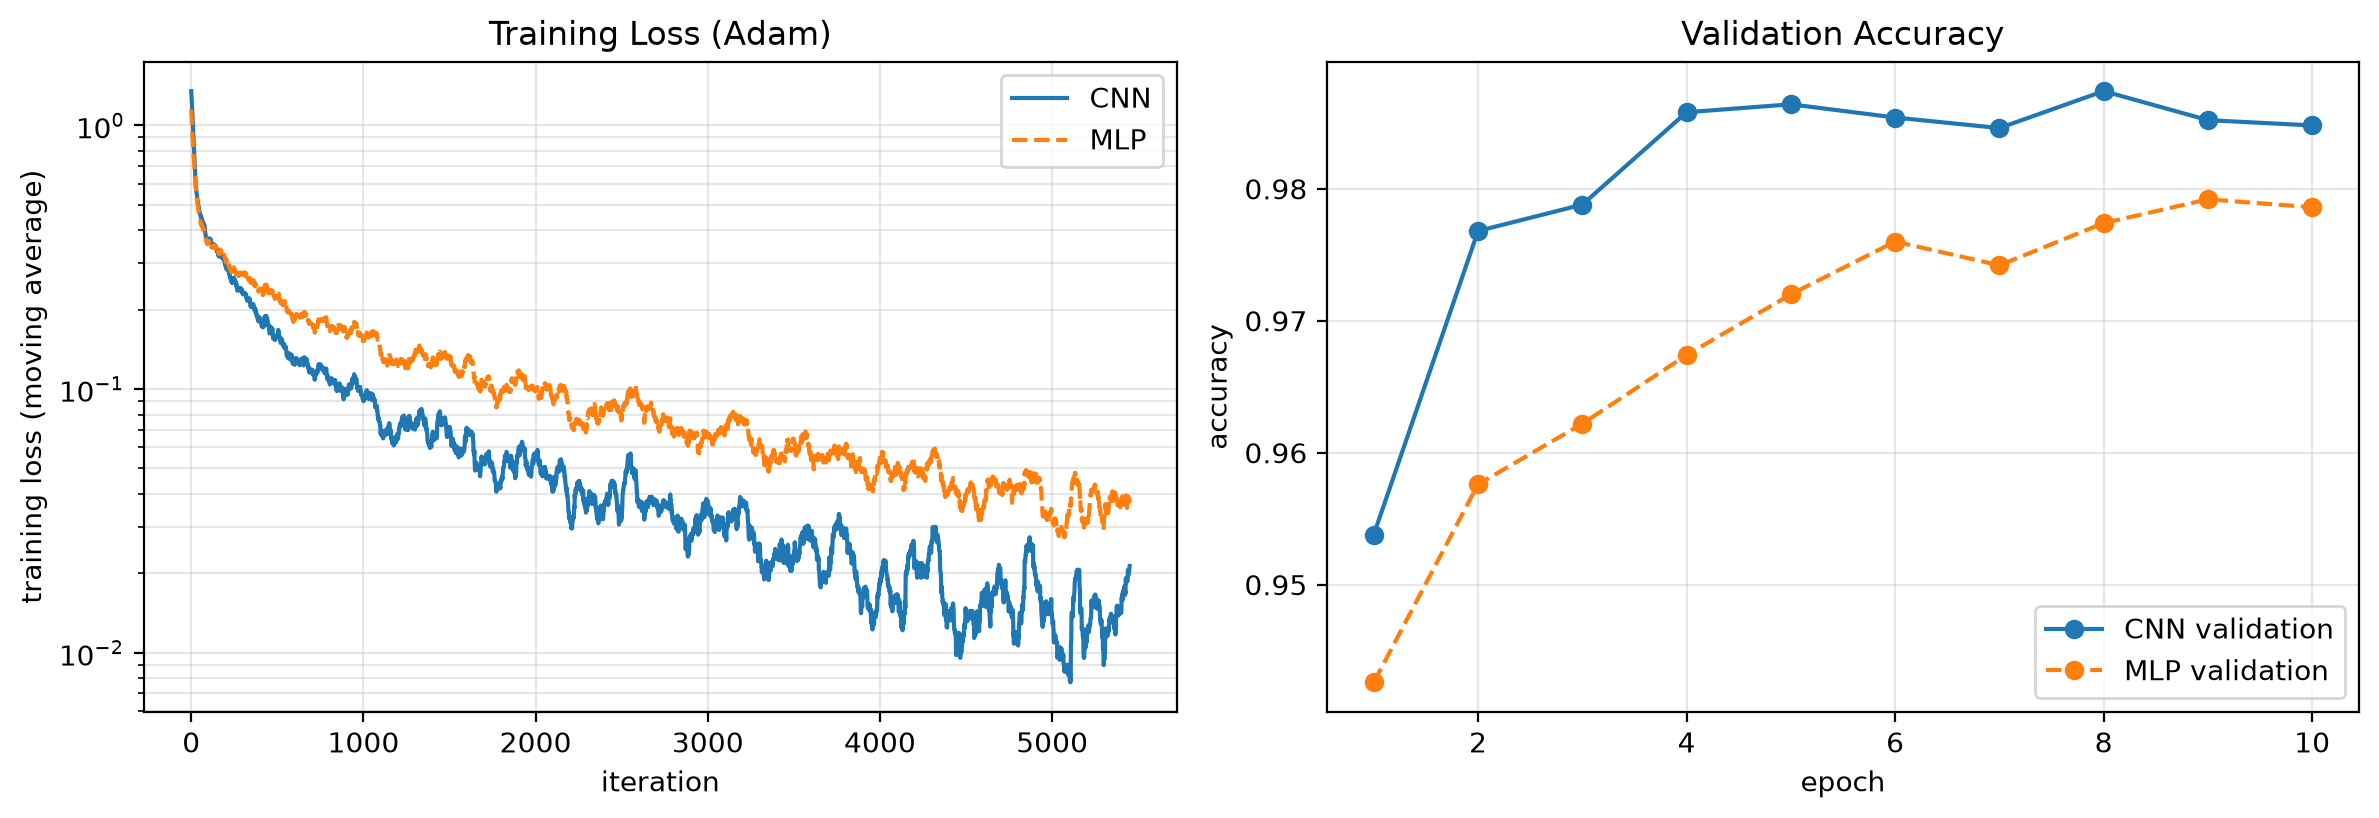
\includegraphics[width=\textwidth]{figures/cnn_mnist.png}

\small SimpleConvNet과 MLP의 훈련 손실 (50 iteration 이동평균, 로그 눈금, 왼쪽)과 epoch별 검증 정확도 (오른쪽)
\end{center}
}{%
\begin{center}
\fbox{\parbox{0.8\textwidth}{\centering\small
[그림 자리] \texttt{figures/cnn\_mnist.png}\\
\texttt{mnist\_cnn.py}를 실행하면 생성된다.}}
\end{center}
}

\begin{center}
{\small
\begin{tabular}{@{}lccccccc@{}}
\toprule
& \multicolumn{4}{c}{검증 정확도} & & & \\
\cmidrule(lr){2-5}
& 1 epoch & 2 epoch & 5 epoch & 10 epoch & 시험 & 매개변수 & epoch당 \\
\midrule
SimpleConvNet & $95.4\%$ & $97.7\%$ & $98.6\%$ & $98.5\%$ & $\mathbf{98.5\%}$ & $433890$ & 약 $60$초 \\
MLP ($784\to100\to10$) & $94.3\%$ & $95.8\%$ & $97.2\%$ & $97.9\%$ & $97.6\%$ & $79510$ & 약 $1$초 \\
\bottomrule
\end{tabular}}
\end{center}

\begin{itemize}[leftmargin=1.8em]
\item CNN은 \textbf{$2$ epoch 만에} 검증 정확도 $97.7\%$로, MLP가 $10$ epoch 동안 도달한 $97.9\%$에 거의 이르고, $4$ epoch부터는 $98.5\%$ 이상을 유지한다.
시험 정확도는 $98.5\%$로 MLP보다 약 $1\%$p 높다. 틀리는 수로 보면 $10000$장 중 $237$장에서 $154$장으로 약 $35\%$ 줄었다.
\item 손실도 CNN이 훨씬 빨리, 훨씬 낮게 내려간다.
\item 다만 매개변수 수가 다르므로 공정한 비교는 아니다. CNN의 매개변수 대부분은 합성곱 계층이 아니라 Affine 계층에 있다.
합성곱 계층의 $780$개 매개변수가 이미지의 모양을 이용해 \textbf{좋은 특징}을 만들어 주기 때문에
뒤의 Affine 계층이 분류를 더 쉽게 하는 것이다.
\item numpy로 구현한 CNN은 한 epoch에 약 $1$분이 걸린다. 합성곱은 계산량이 많아 GPU와 최적화된 라이브러리가 중요하다.
\end{itemize}

$20$ epoch 정도 학습하면 시험 정확도가 약 $99\%$까지 올라간다.
이 노트에서는 시간을 줄이려고 $10$ epoch만 학습하였다.

% =================================================
\section{CNN 시각화하기}\label{sec:visual}
% =================================================

CNN의 합성곱 계층은 무엇을 보고 있을까? 학습된 필터와 그 출력을 그려 본다.

\subsection{첫 번째 층의 가중치 시각화하기}\label{sec:filters}

첫 번째 합성곱 계층의 필터는 $(30,1,5,5)$, 즉 $5\times5$ 크기의 흑백 이미지 $30$장으로 볼 수 있다.
학습 전과 후의 필터를 이미지로 그리면 다음과 같다 (밝을수록 큰 가중치).

\IfFileExists{figures/cnn_filters.png}{%
\begin{center}
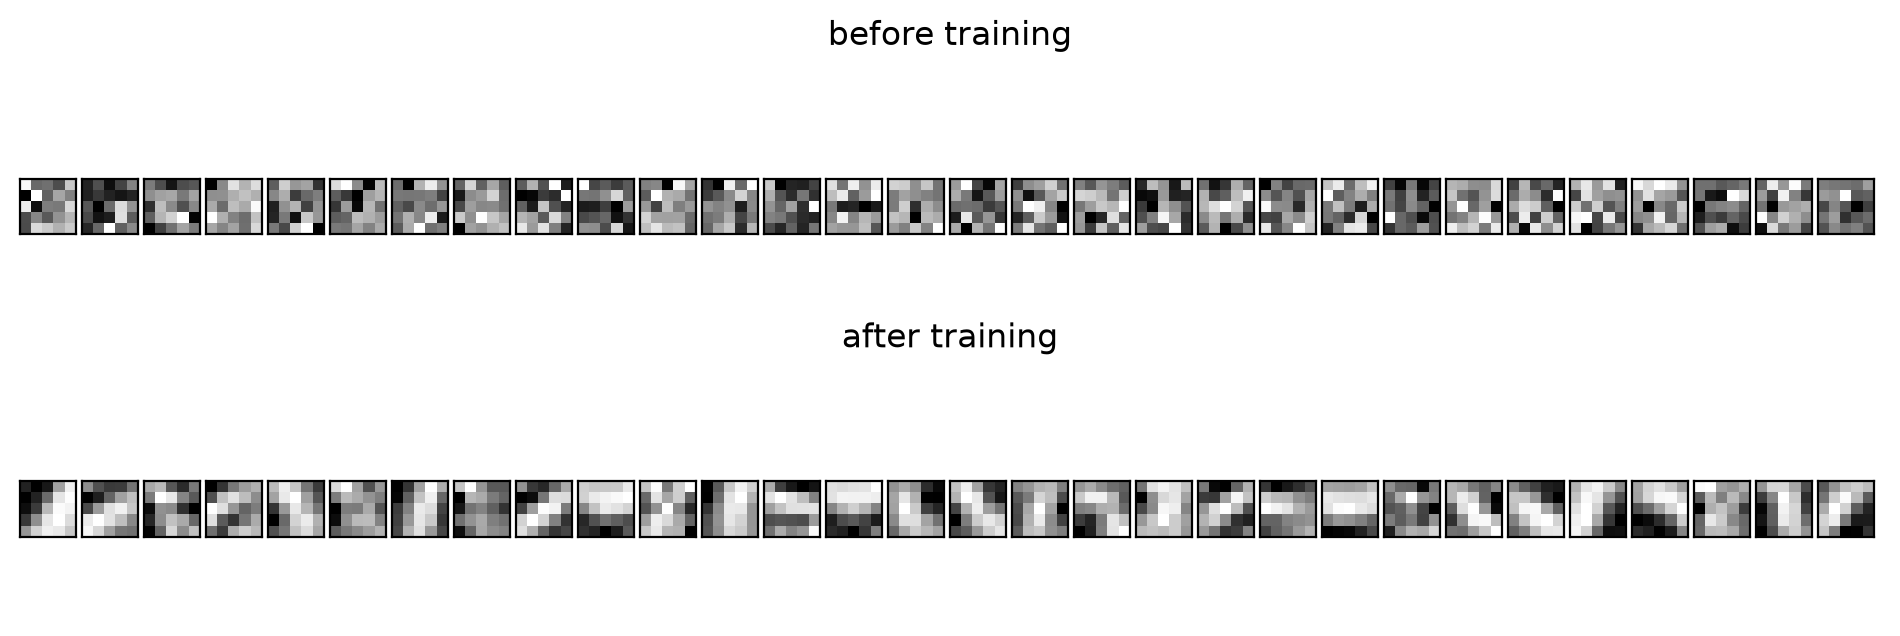
\includegraphics[width=\textwidth]{figures/cnn_filters.png}

\small 첫 번째 합성곱 계층의 필터 $30$개: 학습 전 (위)과 학습 후 (아래)
\end{center}
}{%
\begin{center}
\fbox{\parbox{0.8\textwidth}{\centering\small
[그림 자리] \texttt{figures/cnn\_filters.png}\\
\texttt{mnist\_cnn.py}를 실행하면 생성된다.}}
\end{center}
}

학습 전의 필터는 흑백의 정도가 무작위이지만, 학습 후의 필터는 흰색과 검은색이 \textbf{규칙적으로 나뉜} 모양으로 바뀌었다.
어떤 필터는 왼쪽이 어둡고 오른쪽이 밝으며 (세로 경계), 어떤 필터는 위가 어둡고 아래가 밝고 (가로 경계),
어떤 필터는 대각선 방향으로 밝은 띠가 있다.
흰색에서 검은색으로 바뀌는 경계, 즉 \textbf{에지}에 반응하는 필터가 학습된 것이다.
\ref{sec:conv}절에서 본 Sobel 필터처럼 사람이 설계했던 필터를 network가 데이터로부터 스스로 찾아냈다.

\paragraph{필터는 무엇에 반응하는가: 특징 맵.}
필터 자체보다 필터를 이미지에 적용한 결과, 즉 \textbf{특징 맵}을 보면 필터의 역할이 더 잘 드러난다.
학습된 network의 합성곱 계층에 시험 이미지 하나를 넣어 출력 $(1,30,24,24)$ 중 앞의 $8$장을 그린다.
\begin{lstlisting}
image = x_test[:1]                                     # (1, 1, 28, 28)
feature = cnn.layers[0].forward(image)                 # (1, 30, 24, 24)
\end{lstlisting}

\IfFileExists{figures/cnn_feature_maps.png}{%
\begin{center}
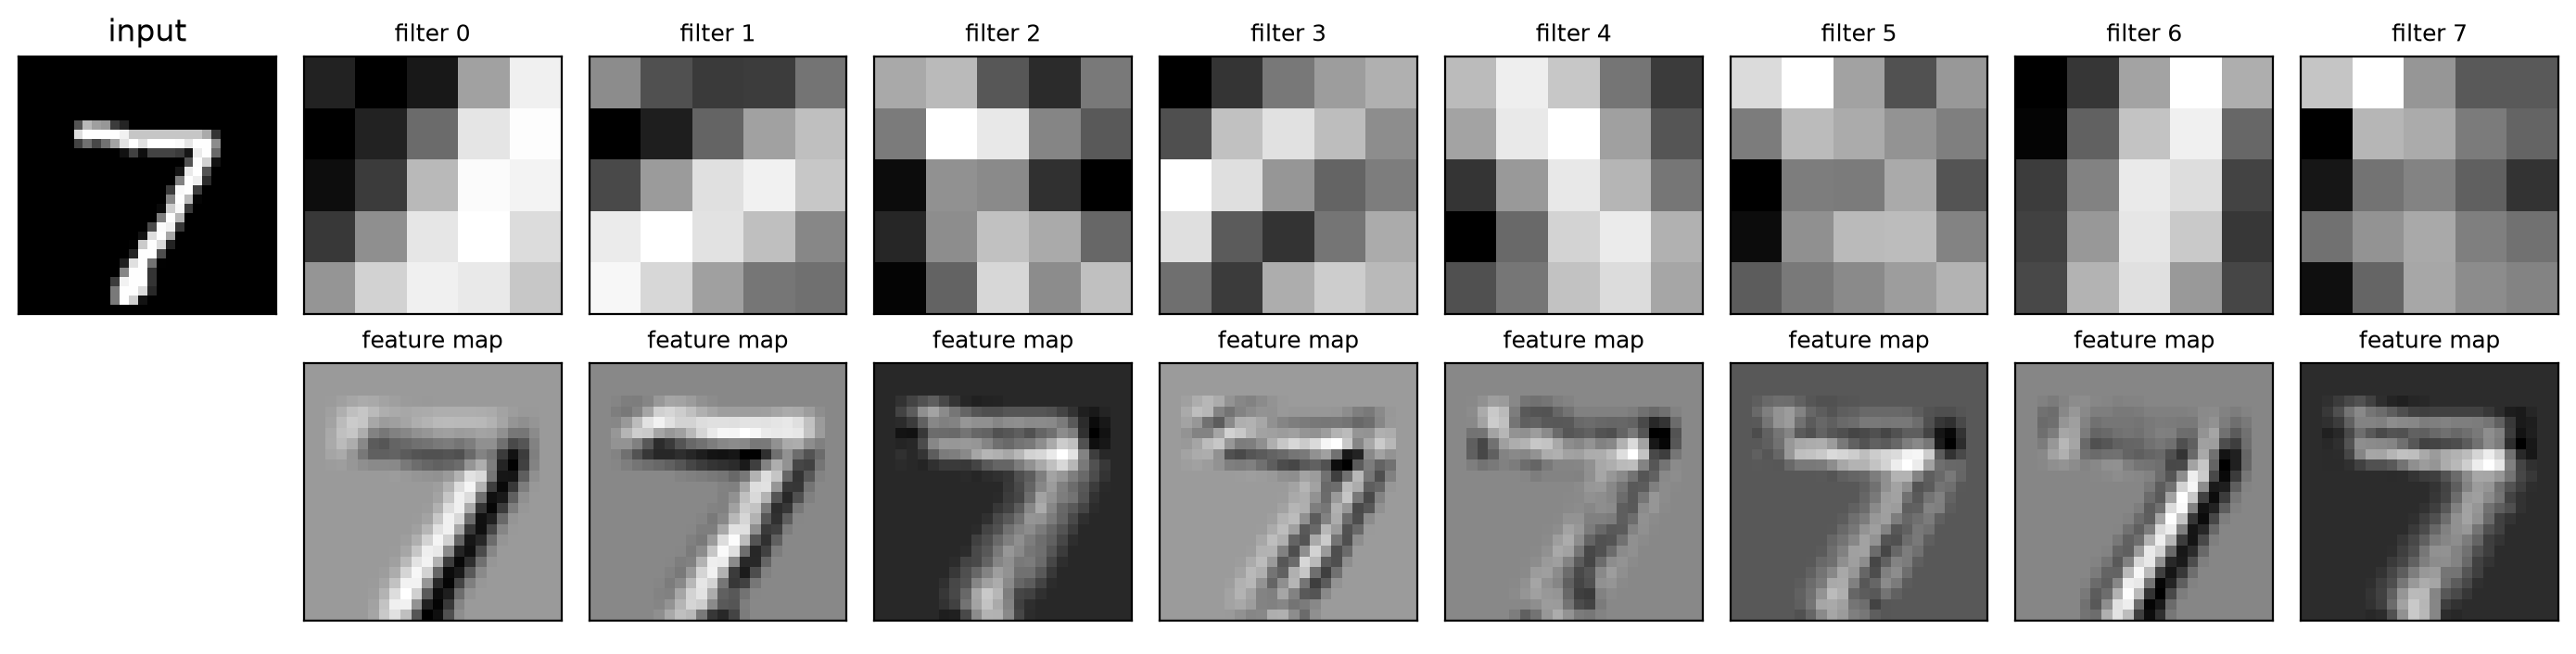
\includegraphics[width=\textwidth]{figures/cnn_feature_maps.png}

\small 입력 이미지와 학습된 필터 $8$개 (위), 각 필터의 출력 특징 맵 (아래, ReLU 적용 전)
\end{center}
}{%
\begin{center}
\fbox{\parbox{0.8\textwidth}{\centering\small
[그림 자리] \texttt{figures/cnn\_feature\_maps.png}\\
\texttt{mnist\_cnn.py}를 실행하면 생성된다.}}
\end{center}
}

\begin{itemize}[leftmargin=1.8em]
\item 특징 맵마다 숫자 7의 \textbf{서로 다른 부분이 밝게}(큰 값) 나타난다.
예를 들어 필터 $0$ (왼쪽이 어둡고 오른쪽이 밝다)은 대각선 획의 왼쪽 가장자리에서 밝고 오른쪽 가장자리에서 어둡다.
필터 $1$ (위가 어둡고 아래가 밝다)은 위쪽 가로 획의 아래 가장자리에 강하게 반응하고,
필터 $6$ (가운데 세로로 밝은 띠)은 대각선 획 자체를 밝게 나타낸다.
\item 즉 첫 번째 층의 필터는 특정 방향의 \textbf{에지}(색이 바뀌는 경계)에 반응한다.
같은 필터를 모든 위치에 적용하므로, 그 방향의 에지가 이미지의 어디에 있든 찾아낸다.
\item 이렇게 만든 $30$장의 특징 맵을 풀링으로 줄인 뒤 Affine 계층이 조합하여 숫자를 판단한다.
\end{itemize}

\subsection{층 깊이에 따른 추출 정보 변화}\label{sec:depth}

첫 번째 층의 필터는 에지나 블롭(blob, 국소적으로 덩어리진 영역) 같은 \textbf{저수준 정보}에 반응한다.
그렇다면 층을 여러 개 쌓으면 어떻게 될까?
대규모 이미지 데이터(ImageNet)로 학습한 $8$층 CNN (AlexNet, \ref{sec:alexnet}절)에서
각 층의 뉴런이 어떤 이미지에 가장 강하게 반응하는지 시각화한 결과는 다음과 같다 (Zeiler와 Fergus, 2014 등).

\begin{center}
\begin{minipage}{\textwidth}\centering
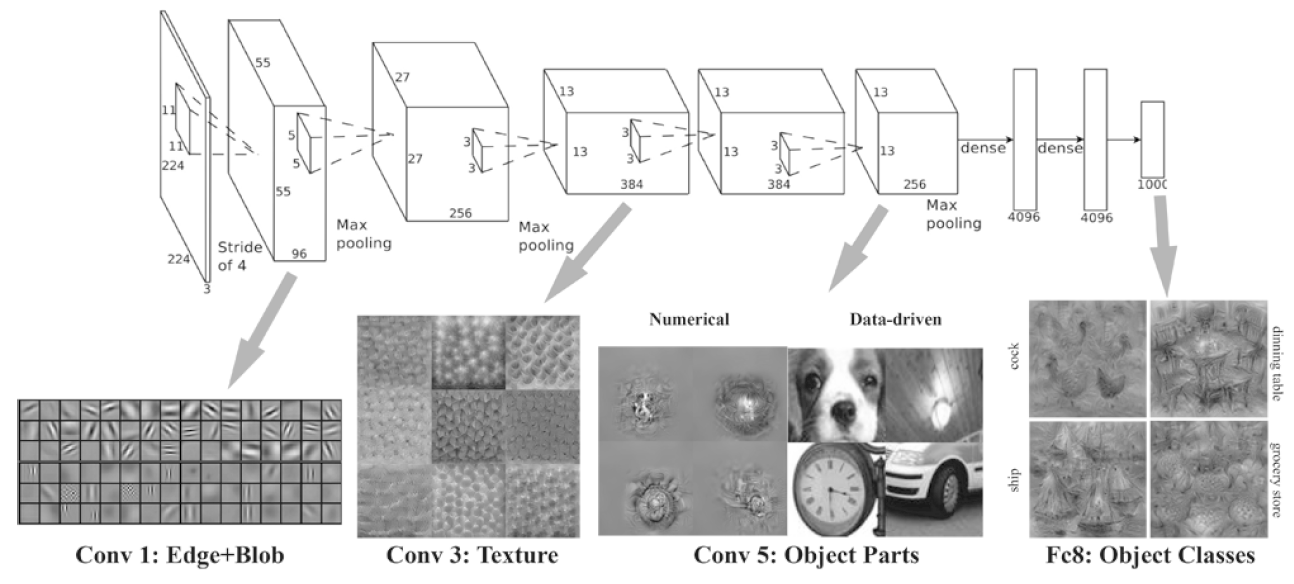
\includegraphics[width=\textwidth]{figures/cnn_depth_layers.png}

\small 층 깊이에 따른 뉴런의 반응 대상. 위는 network의 구조 (합성곱 계층 $5$개 + 완전연결 계층 $3$개),
아래는 각 층의 뉴런이 강하게 반응하는 이미지이다.
\end{minipage}
\end{center}

\begin{itemize}[leftmargin=1.8em]
\item \textbf{Conv 1 (에지와 블롭):} 첫 번째 층의 필터는 여러 방향의 줄무늬와 색 덩어리 모양이다.
앞에서 본 Sobel 같은 에지 필터와 닮았다.
\item \textbf{Conv 3 (텍스처):} 세 번째 층은 에지가 반복된 \textbf{무늬}(벌집, 비늘 같은 질감)에 반응한다.
\item \textbf{Conv 5 (사물의 일부):} 다섯 번째 층은 개의 얼굴, 시계의 문자판, 자동차 바퀴처럼 \textbf{사물의 부분}에 반응한다.
왼쪽(Numerical)은 그 뉴런의 출력이 가장 커지도록 입력 이미지를 계산으로 만든 것이고,
오른쪽(Data-driven)은 실제 데이터 중에서 그 뉴런이 가장 강하게 반응한 이미지이다.
\item \textbf{Fc8 (사물의 클래스):} 마지막 완전연결 계층의 뉴런은 닭, 식탁, 배, 식료품점처럼 \textbf{사물 전체}에 반응한다.
\end{itemize}

즉 층이 깊어질수록 뉴런이 반응하는 대상이 단순한 모양에서 점점 ``고급'' 정보로 바뀐다.
사물의 \textbf{의미}를 이해하는 방향으로 변하는 것이다.
이렇게 \textbf{단순한 특징을 조합하여 점점 추상적인 특징을 만드는 것}이 층을 깊게 쌓는 이유이다.
합성곱 계층을 여러 번 거칠수록 출력의 한 원소가 보는 입력의 범위(\textbf{수용 영역, receptive field})가 넓어지므로,
뒤쪽 층일수록 이미지의 넓은 영역을 보고 판단할 수 있다.

\begin{center}
\begin{tikzpicture}[>=Latex,x=0.62cm,y=1.15cm,
  nd/.style={circle,draw=black!45,fill=white,minimum size=4.2mm,inner sep=0pt},
  hn/.style={circle,draw=orange!80!black,fill=orange!35,very thick,minimum size=4.2mm,inner sep=0pt}]
% (a) 1D: 3 conv layers (filter 3, stride 1) on 9 inputs
\foreach \l in {0,1,2,3} {
  \pgfmathtruncatemacro{\lo}{\l}
  \pgfmathtruncatemacro{\hi}{8-\l}
  \foreach \x in {\lo,...,\hi} {
    \pgfmathtruncatemacro{\d}{abs(\x-4)}
    \pgfmathtruncatemacro{\r}{3-\l}
    \ifnum\d>\r \node[nd] (n\l-\x) at (\x,\l) {}; \else \node[hn] (n\l-\x) at (\x,\l) {}; \fi
  }
}
\foreach \l in {1,2,3} {
  \pgfmathtruncatemacro{\m}{\l-1}
  \pgfmathtruncatemacro{\lo}{\l}
  \pgfmathtruncatemacro{\hi}{8-\l}
  \foreach \x in {\lo,...,\hi} {
    \pgfmathtruncatemacro{\d}{abs(\x-4)}
    \pgfmathtruncatemacro{\r}{3-\l}
    \pgfmathtruncatemacro{\xa}{\x-1}
    \pgfmathtruncatemacro{\xb}{\x+1}
    \ifnum\d>\r
      \foreach \u in {\xa,\x,\xb} \draw[black!20] (n\m-\u) -- (n\l-\x);
    \else
      \foreach \u in {\xa,\x,\xb} \draw[orange!80!black,thick] (n\m-\u) -- (n\l-\x);
    \fi
  }
}
\foreach \l/\t in {0/입력,1/층 $1$,2/층 $2$,3/층 $3$} \node[font=\small,anchor=east] at (-0.6,\l) {\t};
\foreach \l/\w in {1/3,2/5,3/7} \node[font=\small,anchor=west,text=orange!60!black] at (8.6,\l) {보는 입력: $\w$칸};
\draw[decorate,decoration={brace,mirror,amplitude=5pt},thick] (0.7,-0.35) -- (7.3,-0.35)
  node[midway,below=6pt,font=\small] {층 $3$의 한 원소가 보는 입력: $7$칸};
\node[font=\small] at (4,-1.45) {(a) 필터 길이 $3$인 합성곱을 세 번 (1차원)};
% (b) 2D: nested receptive fields on a 9x9 input
\begin{scope}[shift={(13.6,-0.55)},x=0.42cm,y=0.42cm]
\fill[orange!12] (1,1) rectangle (8,8);
\fill[orange!28] (2,2) rectangle (7,7);
\fill[orange!55] (3,3) rectangle (6,6);
\draw[step=1,black!25] (0,0) grid (9,9);
\draw[orange!80!black,very thick] (3,3) rectangle (6,6);
\draw[orange!80!black,very thick,dashed] (2,2) rectangle (7,7);
\draw[orange!80!black,very thick,dotted] (1,1) rectangle (8,8);
\draw[black!60] (0,0) rectangle (9,9);
\draw (6,4.5) -- (10.3,7.5) node[right,font=\small] {층 $1$: $3\times3$};
\draw (7,3.5) -- (10.3,4.5) node[right,font=\small] {층 $2$: $5\times5$};
\draw (8,2.5) -- (10.3,1.5) node[right,font=\small] {층 $3$: $7\times7$};
\node[font=\small] at (6.3,-2.5) {(b) 같은 일을 이미지 (2차원)에서};
\end{scope}
\end{tikzpicture}

\small 뒤쪽 층으로 갈수록 넓어지는 수용 영역. 층 $3$의 원소 하나 (맨 위 주황색)가 입력 $7$칸에 의존한다.
\end{center}

$3\times3$ 필터 (스트라이드 $1$)를 $L$번 쌓으면 수용 영역은 $(2L+1)\times(2L+1)$이 된다.
중간에 $2\times2$ 풀링 (스트라이드 $2$)이 들어가면 그 뒤의 한 칸이 입력의 두 칸에 해당하므로 수용 영역은 훨씬 빨리 넓어진다.
그래서 앞쪽 층은 작은 에지를, 뒤쪽 층은 이미지의 큰 부분이나 전체를 보고 판단할 수 있다.

% =================================================
\section{대표적인 CNN}\label{sec:famous}
% =================================================

CNN의 원조인 LeNet과, 딥러닝이 주목받게 된 계기가 된 AlexNet을 살펴본다.

\begin{remarkbox}[CNN 이전의 문자 인식: 사람이 설계한 특징]
문자 인식(OCR)은 1950년대부터 패턴 인식의 대표 문제였고, 1990년대까지는
\textbf{``사람이 설계한 특징 추출기 + 학습하는 분류기''}가 주류였다.
\begin{itemize}[leftmargin=1.5em]
\item \textbf{템플릿 매칭 (1950--60년대):} 글자마다 표준 모양을 저장해 두고 가장 비슷한 것을 고른다 (템플릿 전체를 하나의 큰 필터로 쓴 셈).
위치, 크기, 글씨체가 조금만 달라도 실패하였다. 기계 판독을 쉽게 하는 \textbf{전용 글꼴}도 만들어졌다
(광학식 판독용 OCR-A, 수표의 자기잉크식 판독용 E-13B).
\item \textbf{사람이 설계한 특징 (1960--90년대):} 방향 필터 (Sobel, Gabor)로 센 가로·세로·대각선 획의 양,
이미지를 구역으로 나누어 센 획의 양 (zoning, 사실상 평균 풀링), 행·열별 픽셀 수, 구멍·끝점·교차점의 개수,
이동과 크기에 변하지 않는 모멘트 등을 뽑아 k-NN, 통계적 분류기, SVM 등에 넣었다.
\item \textbf{한계:} 문자 체계마다 전문가가 특징을 새로 설계하고 조정해야 했고, 손글씨의 다양한 기울기와 굵기에 약했으며,
특징 추출 단계에서 버린 정보는 분류기가 되살릴 수 없었다.
\end{itemize}
LeCun 등은 LeNet 논문 (1998)에서 바로 이 구조를 지적하고, \textbf{특징 추출기까지 데이터로 학습}하자고 제안하였다.
흥미롭게도 학습된 CNN의 첫 층 필터는 방향 에지 필터와 비슷해진다.
사람이 설계한 특징이 틀렸던 것이 아니라, 그 위의 복잡한 조합을 사람이 설계하기 어려웠던 것이다.
\end{remarkbox}

\subsection{LeNet}\label{sec:lenet}

LeNet은 손글씨 숫자를 인식하는 network로 1998년에 제안되었다 (LeCun 등).
합성곱 계층과 풀링 계층(정확히는 \textbf{서브샘플링} 계층: $2\times2$ 영역을 더한 뒤 채널마다 학습하는 계수와 편향을 적용하고 활성화 함수를 통과시킨다)을 반복하고,
마지막으로 완전연결 계층을 거쳐 결과를 출력한다.

\begin{center}
\begin{minipage}{\textwidth}\centering
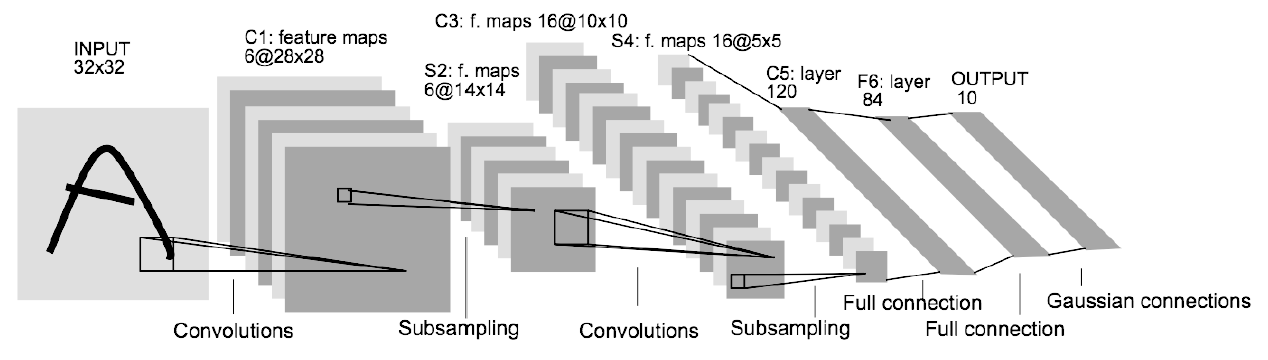
\includegraphics[width=\textwidth]{figures/lenet.png}

\small LeNet-5의 구조 (LeCun 등, 1998). ``$6@28\times28$''은 $28\times28$ 크기의 특징 맵 $6$장이라는 뜻이다.
\end{minipage}
\end{center}

그림의 C는 합성곱(Convolution), S는 서브샘플링(Subsampling), F는 완전연결 계층이다.
C5는 $5\times5$ 입력에 $5\times5$ 필터 $120$개를 적용하여 $1\times1$ 출력 $120$개를 만들므로 사실상 완전연결 계층이다.
마지막 출력 (Gaussian connections)은 지금은 Softmax로 바뀌었다.

\begin{remarkbox}[LeNet의 서브샘플링]
서브샘플링(subsampling)은 ``표본을 줄인다'', 즉 해상도를 낮춘다는 뜻으로, LeNet의 풀링 계층이다.
S2는 C1의 특징 맵마다 겹치지 않는 $2\times2$ 영역 하나에서 출력 하나를 만든다.
\[
y=\sigma\bigl(w\,(x_1+x_2+x_3+x_4)+b\bigr)
\]
네 값을 더하고, 학습하는 계수 $w$를 곱하고 편향 $b$를 더한 뒤, 활성화 함수 $\sigma$ (scaled tanh)를 통과시킨다.
예를 들어 영역이 $\begin{pmatrix}1&3\\2&6\end{pmatrix}$이고 $w=0.25$, $b=0$이면 $0.25\times12=3$으로 네 값의 \textbf{평균}이다.
즉 서브샘플링은 \textbf{평균 풀링 (스트라이드 $2$)}에 학습하는 배율, 편향, 활성화를 덧붙인 것이고, $28\times28$ 특징 맵이 $14\times14$가 된다.
\begin{itemize}[leftmargin=1.5em]
\item \textbf{매개변수:} $w$와 $b$는 특징 맵마다 하나씩이고, 같은 맵의 모든 위치가 공유한다.
S2는 $6\times2=12$개, S4는 $16\times2=32$개이다. 지금의 최대 풀링은 $0$개이다.
\item \textbf{목적:} 손글씨는 쓸 때마다 획의 위치가 조금씩 다르므로, 특징의 정확한 위치는 오히려 방해가 된다.
해상도를 낮추면 위치가 조금 어긋나도 출력이 거의 같다. Hubel과 Wiesel의 복합 세포, Neocognitron의 C층과 같은 역할이다.
\end{itemize}
\end{remarkbox}

\texttt{SimpleConvNet}과 비교하면 거의 같은 구조이지만, 지금의 CNN과는 다음이 다르다.
\begin{itemize}[leftmargin=1.8em]
\item \textbf{활성화 함수}: LeNet은 sigmoid 계열의 함수 (scaled tanh)를 썼다. 지금은 주로 ReLU를 쓴다.
\item \textbf{풀링}: LeNet은 매개변수가 있는 서브샘플링으로 중간 데이터의 크기를 줄였다. 지금은 매개변수가 없는 최대 풀링이 주류이다.
\end{itemize}
그래도 거의 $30$년 전에 이미 지금의 CNN과 같은 기본 구조가 완성되어 있었다는 것이 놀라운 점이다.

\subsection{AlexNet}\label{sec:alexnet}

LeNet 이후 오랫동안 주목받지 못하던 CNN은 2012년 AlexNet (Krizhevsky, Sutskever, Hinton)의 등장으로
딥러닝 열풍을 일으켰다. 대규모 이미지 인식 대회(ILSVRC 2012)에서 top-5 오류율 약 $15\%$로,
$26\%$였던 2위와 큰 차이로 우승하였다.

\begin{center}
\begin{minipage}{\textwidth}\centering
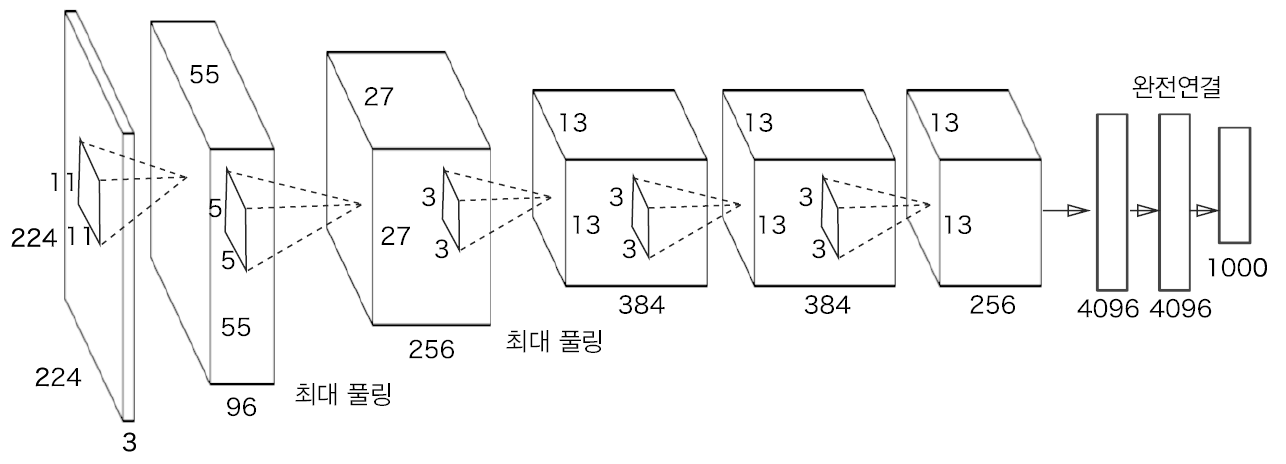
\includegraphics[width=\textwidth]{figures/alexnet.png}

\small AlexNet의 구조 (Krizhevsky 등, 2012): 합성곱 계층 $5$개와 완전연결 계층 $3$개
\end{minipage}
\end{center}

그림의 입력은 원 논문을 따라 $224\times224$로 적혀 있지만, 첫 번째 층 (필터 $11\times11$, 스트라이드 $4$)의 출력 $55\times55$는
입력이 $227\times227$이고 패딩이 $0$일 때 출력 크기 공식과 맞는다 (연습문제 1).

AlexNet은 합성곱 계층과 풀링 계층을 거듭하며 마지막으로 완전연결 계층을 거쳐 결과를 출력한다는 점에서 LeNet과 같지만,
다음과 같은 변화가 있었다.
\begin{itemize}[leftmargin=1.8em]
\item 활성화 함수로 \textbf{ReLU}를 쓴다.
\item LRN(Local Response Normalization)이라는 국소적 정규화를 하는 계층을 쓴다
(지금은 배치 정규화로 대체되었다).
\item \textbf{드롭아웃}을 쓴다 (완전연결 계층).
\item 최대 풀링을 쓴다.
\end{itemize}
매개변수는 약 $6000$만 개이다. 이것을 학습할 수 있었던 것은 네트워크 구조뿐 아니라
\textbf{빅데이터}(ImageNet, 약 $120$만 장의 학습 이미지)와 대량의 병렬 계산을 하는 \textbf{GPU}가 보급된 덕분이다.

\begin{keybox}[AlexNet에는 지금까지 배운 부품이 모두 있다]
ReLU, 최대 풀링, 드롭아웃 (지난 주), 정규화 계층 (배치 정규화의 선배 격), GPU에서의 대규모 행렬곱 (im2col).
그 뒤의 CNN도 같은 부품을 더 깊게 쌓는 방향으로 발전하였다:
VGG (2014, $3\times3$ 합성곱을 쌓아 완전연결 계층 포함 $16\sim19$층), GoogLeNet (2014, 여러 크기의 필터를 병렬로),
ResNet (2015, 입력을 건너뛰어 더하는 skip connection으로 $150$층 이상).
\end{keybox}

% =================================================
\section{PyTorch로 구현하기}\label{sec:torchcnn}
% =================================================

지난 시간에 PyTorch로 완전연결 network를 만들었다.
같은 방법으로 \texttt{SimpleConvNet}을 PyTorch로 만들면, 바뀌는 것은 계층의 이름뿐이다
(\texttt{mnist\_cnn\_torch.py}).
\begin{center}
\begin{tabular}{@{}ll@{}}
\toprule
우리의 구현 (\texttt{conv\_layers.py}) & PyTorch \\
\midrule
\texttt{Convolution(W, B, stride, pad)} & \texttt{nn.Conv2d(C, FN, kernel\_size, stride, padding)} \\
\texttt{Pooling(2, 2)} & \texttt{nn.MaxPool2d(2)} \\
\texttt{Flatten()} & \texttt{nn.Flatten()} \\
필터 \texttt{W}: $(FN,C,FH,FW)$ & \texttt{weight}: $(FN,C,FH,FW)$ (같은 순서) \\
\bottomrule
\end{tabular}
\end{center}
\begin{lstlisting}
model = nn.Sequential(
    nn.Conv2d(1, 30, kernel_size=5),      # (N, 1, 28, 28) -> (N, 30, 24, 24)
    nn.ReLU(),
    nn.MaxPool2d(2),                      # -> (N, 30, 12, 12)
    nn.Flatten(),                         # -> (N, 4320)
    nn.Linear(30 * 12 * 12, 100),
    nn.ReLU(),
    nn.Linear(100, 10),
).to(device)
\end{lstlisting}
데이터는 $(N,1,28,28)$ 모양의 텐서로 만들어 넣는다. 학습 루프는 지난 시간의 코드와 같다.
\begin{lstlisting}
def to_dataset(x, t):
    """images (N, 784) -> (N, 1, 28, 28) tensors, one-hot labels -> class indices"""
    return TensorDataset(torch.tensor(x, dtype=torch.float32).reshape(-1, 1, 28, 28),
                         torch.tensor(np.argmax(t, axis=1)))
\end{lstlisting}

\begin{center}
\begin{tabular}{@{}lcccccc@{}}
\toprule
& \multicolumn{4}{c}{검증 정확도} & & \\
\cmidrule(lr){2-5}
& 1 epoch & 2 epoch & 5 epoch & 10 epoch & 시험 & epoch당 \\
\midrule
numpy (\texttt{conv\_layers.py}) & $95.4\%$ & $97.7\%$ & $98.6\%$ & $98.5\%$ & $98.5\%$ & 약 $60$초 \\
PyTorch (CPU) & $97.6\%$ & $98.4\%$ & $98.6\%$ & $99.1\%$ & $98.8\%$ & 약 $12$초 \\
\bottomrule
\end{tabular}
\end{center}

\begin{itemize}[leftmargin=1.8em]
\item 같은 구조, 같은 optimizer이므로 결과가 비슷하다. 초깃값과 미니배치 순서가 다르므로 숫자가 똑같지는 않다.
\item 같은 CPU에서 PyTorch가 약 $5$배 빠르다. PyTorch는 합성곱을 C++로 최적화된 라이브러리로 계산하며,
GPU가 있으면 \texttt{device="cuda"}만으로 더 빨라질 수 있다 (얼마나 빨라지는지는 환경에 따라 다르니 직접 재 보자).
\item PyTorch의 \texttt{nn.Conv2d}는 기본 초깃값으로 균등분포 (범위 $\pm1/\sqrt{25}$)를 쓴다.
학습된 필터에서 여러 방향의 에지 모양을 볼 수 있다.
\end{itemize}

\IfFileExists{figures/cnn_torch_filters.png}{%
\begin{center}
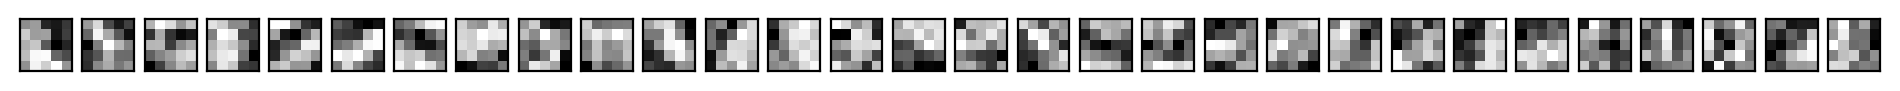
\includegraphics[width=\textwidth]{figures/cnn_torch_filters.png}

\small PyTorch로 학습한 첫 번째 합성곱 계층의 필터 $30$개 (\texttt{model[0].weight})
\end{center}
}{%
\begin{center}
\fbox{\parbox{0.8\textwidth}{\centering\small
[그림 자리] \texttt{figures/cnn\_torch\_filters.png}\\
\texttt{mnist\_cnn\_torch.py}를 실행하면 생성된다.}}
\end{center}
}

% =================================================
\section{정리}\label{sec:summary}
% =================================================

\begin{keybox}[합성곱 신경망: 정리]
\begin{itemize}[leftmargin=1.5em]
\item CNN은 지금까지의 신경망에 \textbf{합성곱 계층}과 \textbf{풀링 계층}을 더한 것이다.
\item 합성곱 계층은 이미지의 \textbf{형상을 유지}하며, 같은 필터를 모든 위치에 적용한다 (가중치 공유).
출력 크기는 $OH=\lfloor\frac{H+2P-FH}{S}\rfloor+1$.
\item 필터는 4차원 $(FN,C,FH,FW)$, 데이터는 4차원 $(N,C,H,W)$이다.
\item 풀링 계층은 매개변수 없이 공간 크기를 줄이며, 작은 위치 변화에 강하다.
\item \textbf{im2col}을 쓰면 합성곱은 하나의 행렬곱, 즉 Affine 계층이 된다. 역전파는 Affine의 역전파와 col2im이다.
\item 첫 층의 필터는 에지와 블롭에 반응하고, 층이 깊어질수록 더 추상적인 정보를 추출한다.
\item LeNet (1998)과 AlexNet (2012)이 대표적인 CNN이며, 빅데이터와 GPU가 딥러닝 발전의 큰 원동력이었다.
\end{itemize}
\end{keybox}

% =================================================
\section{연습문제}
% =================================================

\begin{enumerate}[label=\arabic*.]

\item 다음 합성곱 계층의 출력 크기를 구하라.
(a) 입력 $(32,32)$, 필터 $(5,5)$, 패딩 $2$, 스트라이드 $1$.
(b) 입력 $(227,227)$, 필터 $(11,11)$, 패딩 $0$, 스트라이드 $4$ (AlexNet의 첫 번째 층).
(c) 입력 $(28,28)$에 $2\times2$ 최대 풀링 (스트라이드 $2$)을 두 번 적용한 결과.

\item 입력 $\begin{pmatrix}1&0&2&1\\0&3&1&0\\2&1&0&4\\1&0&1&2\end{pmatrix}$에
필터 $\begin{pmatrix}1&0\\0&-1\end{pmatrix}$를 스트라이드 $1$, 패딩 $0$으로 적용한 결과를 손으로 계산하라.
같은 입력에 $2\times2$ 최대 풀링 (스트라이드 $2$, 패딩 $0$)을 적용한 결과도 구하라.

\item RGB 이미지 ($C=3$)에 $3\times3$ 필터 $64$개를 쓰는 합성곱 계층의 매개변수(가중치와 편향) 수를 구하라.
입력이 $(3,32,32)$이고 패딩 $1$일 때, 같은 크기의 출력 $(64,32,32)$을 완전연결 계층으로 만든다면 가중치는 몇 개가 필요한가?

\item 2번 문제의 최대 풀링에서 출력 쪽 gradient가 $\begin{pmatrix}1&2\\3&4\end{pmatrix}$일 때,
입력 쪽 gradient ($4\times4$)를 구하라.

\item 길이 $5$인 1차원 입력 $(x_1,\ldots,x_5)$에 길이 $3$인 필터를 스트라이드 $1$로 적용하면 출력은 $3$개이다.
im2col 행렬 ($3\times3$)을 쓰고, $x_3$이 몇 번 등장하는지 세어 보라.
이로부터 col2im에서 gradient를 \textbf{더해야} 하는 이유를 설명하라.

\item SimpleConvNet의 합성곱 계층에 패딩 $2$를 주도록 고쳐 보라.
\texttt{conv\_out}, \texttt{pool\_out}, \texttt{flat}은 각각 얼마가 되는가?
Convolution 계층에 \texttt{pad}를 넘기는 부분과 \texttt{flat}의 계산을 고친 뒤,
\texttt{conv\_basics.py}의 gradient 확인으로 검증하라.

\item \texttt{mnist\_cnn\_torch.py}를 고쳐 LeNet과 비슷한 network
(Conv $5\times5$ $6$개, 패딩 $2$ $\to$ ReLU $\to$ MaxPool $\to$ Conv $5\times5$ $16$개 $\to$ ReLU $\to$ MaxPool $\to$ FC $120$ $\to$ ReLU $\to$ FC $84$ $\to$ ReLU $\to$ FC $10$)를 만들고 학습시켜라.
각 계층을 지난 뒤의 shape을 표로 정리하고, 매개변수 수와 검증 정확도를 SimpleConvNet과 비교하라.

\end{enumerate}

\end{document}
